\section{Introduction} 
\label{sec:1-introduction} 
Improving the state's ability to tax effectively is increasingly seen as central to the development process, and the value added tax (VAT) has been proposed as a key tool towards accomplishing this goal.\footnote{\cite{besley2013taxation}.} However, micro-empirical evidence on its effectiveness is relatively limited.\footnote{\citet{almunia2018under}, \cite{naritomi2013consumers}, \cite{Carrilloetal:2017} and \cite{pomeranz2015no} discussed below are notable exceptions. See \cite{Ebrilletal:2001} for an overview of the more aggregate cross-country evidence on the effectiveness of the VAT.}

VAT is a broad-based tax remitted at multiple stages of production (and distribution) with taxes paid on purchases (inputs) credited against taxes withheld on sales (output). In its most common form (known as the ``invoice credit'' method) firms withhold taxes on sales (output tax) from which they deduct the taxes they have already paid on purchases (input credits), and finally remit the difference to the tax authority. Thus, tax revenue is collected, by the tax authority, throughout the production chain (unlike a retail sales tax) but without distorting production decisions (unlike a turnover tax).\footnote{See \cite{ITD2005} for more details.}

The VAT system requires both parties of a transaction to report on it separately. The parties, however, face opposed incentives: the buyer has an incentive to report the transaction -- in order to receive input credit and reduce her tax liability -- while the seller's incentive is to lower her tax liability by not reporting the
transaction. Such opposed incentives are believed to limit the likelihood of collusion between buyer and seller. These multiple reports also enable ``third-party verification'' in that the tax authority can compare buyer reports against seller reports while inspecting returns. This is often cited as a key advantage of the VAT. In
practice, however, there may be significant differences in the ease with which the tax authority can verify third-party reports. For instance, as is true in the initial period of our study, the tax authority may only be able to verify third-party reports after instituting (costly and rare) audits in a lengthy multi-stage process.

In this paper we evaluate the effect of a policy that significantly eased the Delhi tax authority's ability to implement third-party verification. Delhi adopted the VAT in 2005 but until 2012 (year 3 of our data) firms were only required to file a single aggregated return (known as a consolidated return). The consolidated return contained no information on transactions at the firm level so that the tax authority could not match buyer and seller reports directly. Any matching across buyers and sellers could only be done by initiating an audit
and requesting this information from the audited firm and all firms it had interacted with over the relevant tax-period.\footnote{The lack of automatic cross-checking of reports appears to be a common feature of VAT systems. For instance, this was true of the VAT system in Chile discussed in \cite{pomeranz2015no}.  To the best of our knowledge, this seems to be the case in other countries as well -- e.g. tax authorities in Tanzania and Senegal do not systematically collect transaction level information. \cite{Carrilloetal:2017} note that the tax authorities in Ecuador only began to collect sales and purchase data from tax-payers in 2007 and only began cross-checking reports for revenue discrepancies in 2011. \citet{almunia2017analysis} note that while tax authorities in Uganda collect transaction level information, the information is not used in any systematic manner for cross-checking reports.}

Starting in the first quarter of 2012-13 all firms were mandated to file additional, detailed information about transactions with other firms. Specifically, firms were required to provide information, at the firm level, on all purchases and sales and provide tax-identification numbers for all transacting firms. The tax authority could now (and did) relatively easily cross-check information provided by buyers with the corresponding information from sellers, directly on its own servers, without initiating an audit. In case of a mismatch, notices are automatically generated and sent out to both firms who are then required to amend their respective returns.\footnote{After a mismatch notice is generated, firms are given up to a year to resolve the mismatch. If still unresolved, an assessment is manually carried out by an inspector. While the policy is a significant improvement over previous practice, reconciling mismatches is still a somewhat lengthy process. The nationwide Good and Services Tax (GST), which launched on July 1, 2017, is supposed to further streamline this process. Under the GST regime, if mismatches are not resolved within 180 days all relevant input tax credits will be canceled.}  These notifications mark the first time that third-party information was used in a systematic way by the Delhi tax authority and is likely to be adopted in other VAT regimes as they move towards electronic return filing.

The intended goal of the policy was to reduce evasion by reducing input credit claims and by increasing output tax withholdings. However, whether this will be the case is \emph{ex-ante} unclear since firms can collude (e.g by co-ordinating on off-the-book transactions) to ensure matching reports, thereby subverting third-party verification.\footnote{As has been noted, see e.g. \cite{pomeranz2015no}, the VAT system of third-party verification breaks down at the last step since sales to final customers are not subject to third-party verification. More generally, the system can potentially unravel upwards from any firm which is significantly under-reporting revenues. In our setting third-party verification can break down at most nodes in the chain since registered firms regularly interact with unregistered firms.} Furthermore, since many firms are unregistered, i.e. do not file returns, registered firms can under- or over-report (or otherwise manipulate) transactions with such firms without the fear of being uncovered by third-party verification.\footnote{In effect this means that net revenue disclosed to the authorities at every node is a choice variable. While there is no systematic evidence on the extent of corporate tax-evasion in India, anecdotal evidence suggests that it is high.}

We attempt to understand the effects of this policy reform by focusing on comparisons between wholesale and retail firms. Both wholesalers and retailers face comparable incentives on the purchase side -- they can claim input credit only for purchases from registered firms and post-reform the tax authority automatically verifies these claims against the corresponding counter-claims. However, by virtue of being higher up in the production chain, a wholesaler is more likely to sell to registered firms whereas a retailer is more likely to sell to final customers from whom no verification is possible.\footnote{See \cite{naritomi2013consumers} for an innovative program in Brazil that attempted to address this problem with final customers. Note that in our setting final customers are observationally indistinguishable from unregistered firms. In \cref{fig:salesregistered} we provide evidence for the claim that retailers are more likely to sell to final customers.} Therefore, on the output side, the VAT self-enforcement and third-party verification mechanisms are more likely to break down for retailers relative to wholesalers. As a result, we would expect the policy to have a stronger effect on wholesalers relative to retailers. Our findings are consistent with this hypothesis. Using a difference-in-difference strategy we show that the policy led to a 29\% increase in average tax collections from wholesalers relative to retailers in real terms. This increase was largely driven by an increase in output taxes collected by wholesalers with no differential reduction in input credits.

However, focusing on averages masks significant heterogeneity in the effect of the policy. Treatment effects are substantially higher for larger wholesalers (relative to large retailers) ranked by tax remitted at baseline. A potential explanation lies in the structure of the tax authority monitoring mechanism and the low compliance environment. 96\% of the top one percent of wholesalers are monitored by a special tax assessment unit which focuses solely on high taxpayers. We do not find a comparable increase in tax collections for the top one percent of retailers -- 80\% of whom are also monitored by the same unit. However, unlike wholesalers the bulk of these retailers' sales are to unregistered firms. This suggests that targeted state capacity by itself may be insufficient but when combined with increased information can improve collections even in a low compliance environment.

The remainder of this paper is as follows: \Cref{sec:1-literature} reviews the relevant literature, \cref{sec:conceptual} summarizes  a theoretical framework for understanding the empirics as well as some background on the VAT in Delhi and the policy change of interest, \cref{sec:1-data} describes the data, and \cref{sec:empirical_strategy} describes the empirical strategy and the assumptions underlying our causal claims. \Cref{sec:1-results} presents our results. \Cref{sec:1-mechanism} explores likely mechanism for our reduced form results and \cref{sec:1-conclusion} concludes.

\section{Related Literature} 
\label{sec:1-literature} 
Researchers have argued that VAT is harder to evade than a general sales tax for at least three reasons.\footnote{See e.g. \cite{agha1996designing}.} First, as pointed out earlier, both input sellers and intermediate good purchasers maintain reports of transactions. In principle, this provides a reliable audit trail and serves as a form of third-party verification and should act as a preventive deterrent for firms. Second, the diametrically opposed incentives between buyer and seller should reduce the scope for collusion in these reports. Finally, taxes are remitted at all stages of production rather than only at the retail level and this is thought to render VAT less vulnerable to evasion relative to taxation at a single point (e.g with a sales tax). These arguments have proved compelling to policy makers and VAT has expanded rapidly world-wide with more than 160 countries currently deploying this system. India introduced it in 2005. There is also now a fledgling micro-economic literature that seeks to evaluate the effectiveness of the VAT and its various hypothesized mechanisms.

In an influential paper, \cite{pomeranz2015no} reports results from a randomized experiment in Chile that increases the perceived audit probability for a group of treatment firms. She finds that the treatment had a much smaller effect on firms with paper trails relative to firms without such trails (who would correspond to retailers in our context). We view our work as complementary to this study in several ways. First, Pomeranz's experiment holds the tax authority's information set constant while increasing the audit probability (or the firms perception of the probability), while our study holds the audit probabilities constant changing instead the information set available to the tax authority and firms' knowledge of this.\footnote{In terms of cross-checking ability the Chilean tax-regime was the same as the pre-policy regime in Delhi. The Chilean tax authority could only cross-check buyer and seller reports accurately via an audit (except for a small fraction of firms filing on-line).} \footnote{With the caveat that firms in our study realized that they would have to co-ordinate on reports in order to avoid a mis-match report.}  Second, as Pomeranz notes, Chile has one of the highest tax compliance rates world-wide, while our study takes place in a low compliance environment. This difference in contexts potentially helps explain some of the differences in our results - e.g. for larger firms - as we discuss below. Third, the policy change in our study is a permanent change in the tax-regime which may result in different firm responses compared to a one-time targeted intervention and we can examine the resulting changes over a two-year horizon.

Our work is also related to the recent literature on third-party verification. \cite{kleven2011unwilling} show that evasion rates in Denmark are significant (approximately 40\%) for income that is non third-party verifiable and extremely low for income that is third-party verifiable. In an earlier paper, \citet{slemrod2001taxpayer} find that audit threat letters increase tax payments in Minnesota with the results driven by tax-payers with income that is difficult to verify from a third party (e.g. self-employment or farm income). In our context, firm interactions with other registered firms in both the pre- and post-policy periods are \emph{sensu stricto} third-party verifiable. However, the act of third-party verification is automated in the post-period and our results show that this automation differentially affected firms that reported more third-party verifiable transactions. \citet{Carrilloetal:2017} find that Ecuadorian firms increase reported revenues when informed about revenue discrepancies (based on third-party verification exercises undertaken by the tax authority). However, they also increase (non third-party verifiable) reported costs by 96 cents for every dollar of increased reported revenue. As a result, the verification exercise results in only a minor increase in tax collections.  Similarly, \citet{slemrod2015does} finds that providing credit card sales information for sole-proprietorships to the IRS increased reported revenues by 24\%. However, taxpayers offset the increased revenue reports by increasing reported expenses -- which are harder to third-party verify -- and thereby reduced taxable income.\footnote{See also \cite{kumler2012enlisting} for an empirical study that documents improvements in payroll tax compliance by firms as a result of a policy change that established a closer link between firm reported wages and pensions.} In our setting, non third-party verifiable purchases cannot reduce tax liabilities so such direct strategies are not possible although we do find some evidence consistent with collusion between some firms that has the same effect.

Our findings are also consistent with the theoretical model in \cite{kleven2016can} in that the effects of the improved verification are most pronounced for larger wholesale firms.\footnote{Although the model in \cite{kleven2016can} is described in terms of collusion between workers and firms, the logic extends to collusion between firms; we discuss the relationship in greater detail in \cref{sec:conceptual}.} Our findings of differential effects for larger wholesale firms are also complementary to the larger bunching effects documented in \citet{almunia2018under} for Spanish firms with more third-party verifiable transactions.

\todo[inline, caption={For AM: \citet{almunia2018under} description}]{I think you mean "more" third party verifiable transactions? But then how is it complementary?}

A common theme in this literature is that firms are often able to circumvent monitoring policies by changing behavior along margins not visible to the authorities. Therefore, the eventual intended effect of
the monitoring policy on tax collections is relatively muted.  Our work is related to this literature since the policy change we examine has differential effects on firms whose activities are less visible to the authorities relative to firms whose transactions are more visible and that in addition firms can use a margin unavailable in
high-compliance environments - making off the book transactions.

We also contribute to a recent literature exploring mechanisms to improve the state's tax collection ability.\footnote{See e.g. \cite{gordon2009tax}, \cite{khan2016tax}.} Finally, our work is also relevant to the literature that attempts to understand the role of technology in improving governance in developing countries.\footnote{See e.g. \cite{banerjee2016governance}, \cite{muralidharanetal:2016}, and the review in \cite{finan2017personnel}.}

\section{Conceptual Framework}
\label{sec:conceptual}

We organize our thinking around conceptual framework provided by \cite{allinghamsandmo:1972,kleven2011unwilling} for understanding the differential effects of the policy reform on wholesale and retail firms and \cite{kleven2016can} for understanding the larger effects on bigger wholesale firms.

\cite{kleven2011unwilling} adapt the canonical \cite{allinghamsandmo:1972} model of tax-compliance to incorporate
third-party verifiable income. The model derives the firm's optimal choice of reported income which in turn determines the (endogenized) evasion detection probability. The key trade-off here is balancing the gains arising from tax evasion by reducing reported income against the increase in the probability of detection which is assumed to be an increasing function of the tax evaded. Further, the probability of detection is assumed to be close to one for any evasion of third-party verifiable income but significantly lower for non third-party verifiable income. Consequently, tax-payers will set reported income to be at least as high as their third-party verifiable income and will under-report the non third-party verifiable component of income.

An implication of this model is that an increase in third-party verifiable income will lead to an increase in reported income.\footnote{The setting here differs from the version of the Allingham-Sandmo model exposited in e.g. \cite{Carrilloetal:2017} in that non-third-party verifiable purchases are not eligible for input-tax credit. This difference implies that in our setting firms will not have an incentive to respond to an increase in third-party
reported sales by increasing non-third party verifiable purchases. It is possible for firms to reduce their tax liability by colluding with suppliers to increase their input tax credits. We examine this possibility in the results section below.} Within the model we interpret the automation of cross-checking buyer and seller reports as an increase in third-party verifiable income. However, the increase is larger for wholesale firms because they interact with a larger number of registered firms relative to retail firms.\footnote{Shown in \cref{fig:salesregistered}.} The model then predicts that, ceterus paribus, collections should increase more for wholesale firms relative to retail firms. As we shall see, tax collections from retail firms are relatively unaffected by the reform and we discuss the implications of that finding in the context of this model below.

This previous model takes third-party verifiable income as exogenously given. A complementary framework is provided by \cite{kleven2016can} who examine the choice of how much third-party verifiable income a firm will report in the context of a cooperative game played by (potentially) colluding firms.\footnote{The model is intended to describe the strategic considerations involved in third-party reporting of employee wages by (a) the employer and (b) employees to the tax authority. However, with a suitable caveat, discussed below, it can be adapted to examining third-party reporting between firms.} In the model, a given (henceforth the index) firm interacts with $N$
other firms in a pairwise manner and each pair decides on a common report to be reported separately by each member to the tax-authority. Each member of the pair knows whether the agreed upon report is true. If the (common) reported transaction differs from the truth, then a mismatch report is filed with a certain probability
(that is constant across pairs) to the tax-authority.\footnote{The reasons for the whistle-blowing report are left unmodeled but could represent for instance a breakdown in collusion, disgruntlement, error or moral concerns.} Such denouncement events are assumed to be independent across pairs. It then follows that the likelihood of being denounced is increasing in $N$. \cite{kleven2016can} then show that evasion is decreasing in $N$. The key insight here is that for a index firm, collusion is harder to maintain when interacting with more firms.
\todo[inline, caption={For AM: denouncmenent}]{While I agree that denouncement is increasing in N, i still do not see the connection. Even if firm i denounces, it does not have an effect on n-1 transactions.}


As pointed out earlier, collusion, and hence evasion, under a VAT is harder since the seller and the buyer face opposing incentives. However, if sales can be under-reported at any node in the VAT chain, then collusion becomes feasible at all nodes above the under-reporting node. The basic logic is that under-reporting sales reduces the
strength of the opposing incentives between the under-reporting firm and its suppliers, allowing for collusion.\footnote{See e.g. section 1.2 in \cite{pomeranz2015no}.} In particular, the declines in tax liability via reducing reported sales can now be traded-off against the declines in input tax credit from reducing reported purchases. The firm under-reporting sales and its buyer have some scope for reaching an agreement on reducing reported purchases to the tax authority. This same logic can then be extended up the VAT chain so that all nodes
above can collude and evade taxes even in the presence of third-party reporting.

In high compliance environments, the under-reporting of sales is assumed to occur only at the point of sale to the final consumer since no third-party verification is possible at that final node. However, in Delhi, the majority of our study firms make some sales that are not third-party verifiable. This is because sales to unregistered firms --
i.e. firms that are not registered with the tax authority and hence do not have to file returns-- occur at all nodes of the VAT chain.\footnote{In our study approximately 75\% of firms make some positive sales to unregistered firms.} Therefore, firms have the potential to under-report sales at all nodes on the VAT chain. This in
turn implies that in our context the pairwise analysis of \cite{kleven2016can} can be applied to any two adjacent nodes in the VAT chain. In particular, the pairwise analysis does not depend upon collusion further down the chain (upto the final sale to consumer) as is required in accounts of VAT break-down in high compliance environments.

This interpretation of the model implies that collusion, and hence tax-evasion under third-party reporting will be lower for firms that interact with a larger number of registered firms. Wholesale firms on average interact with more registered firms measured both in terms of number of firms interacted with as well as the fraction of sales that are made to registered firms when compared to retail firms. Based on the model, we hypothesize then that tax collections should increase more for wholesalers following the introduction of effective automated third-party verification.

\todo[caption={For SM: do the regression based on number of interactions}, inline, color=green]{Verify empirically what is going on on the margin of number of firms interacted with the index firm.}




\subsection{Illustrative Example}
\label{subsec:background}

\begin{figure}[t!] 
%\centering
 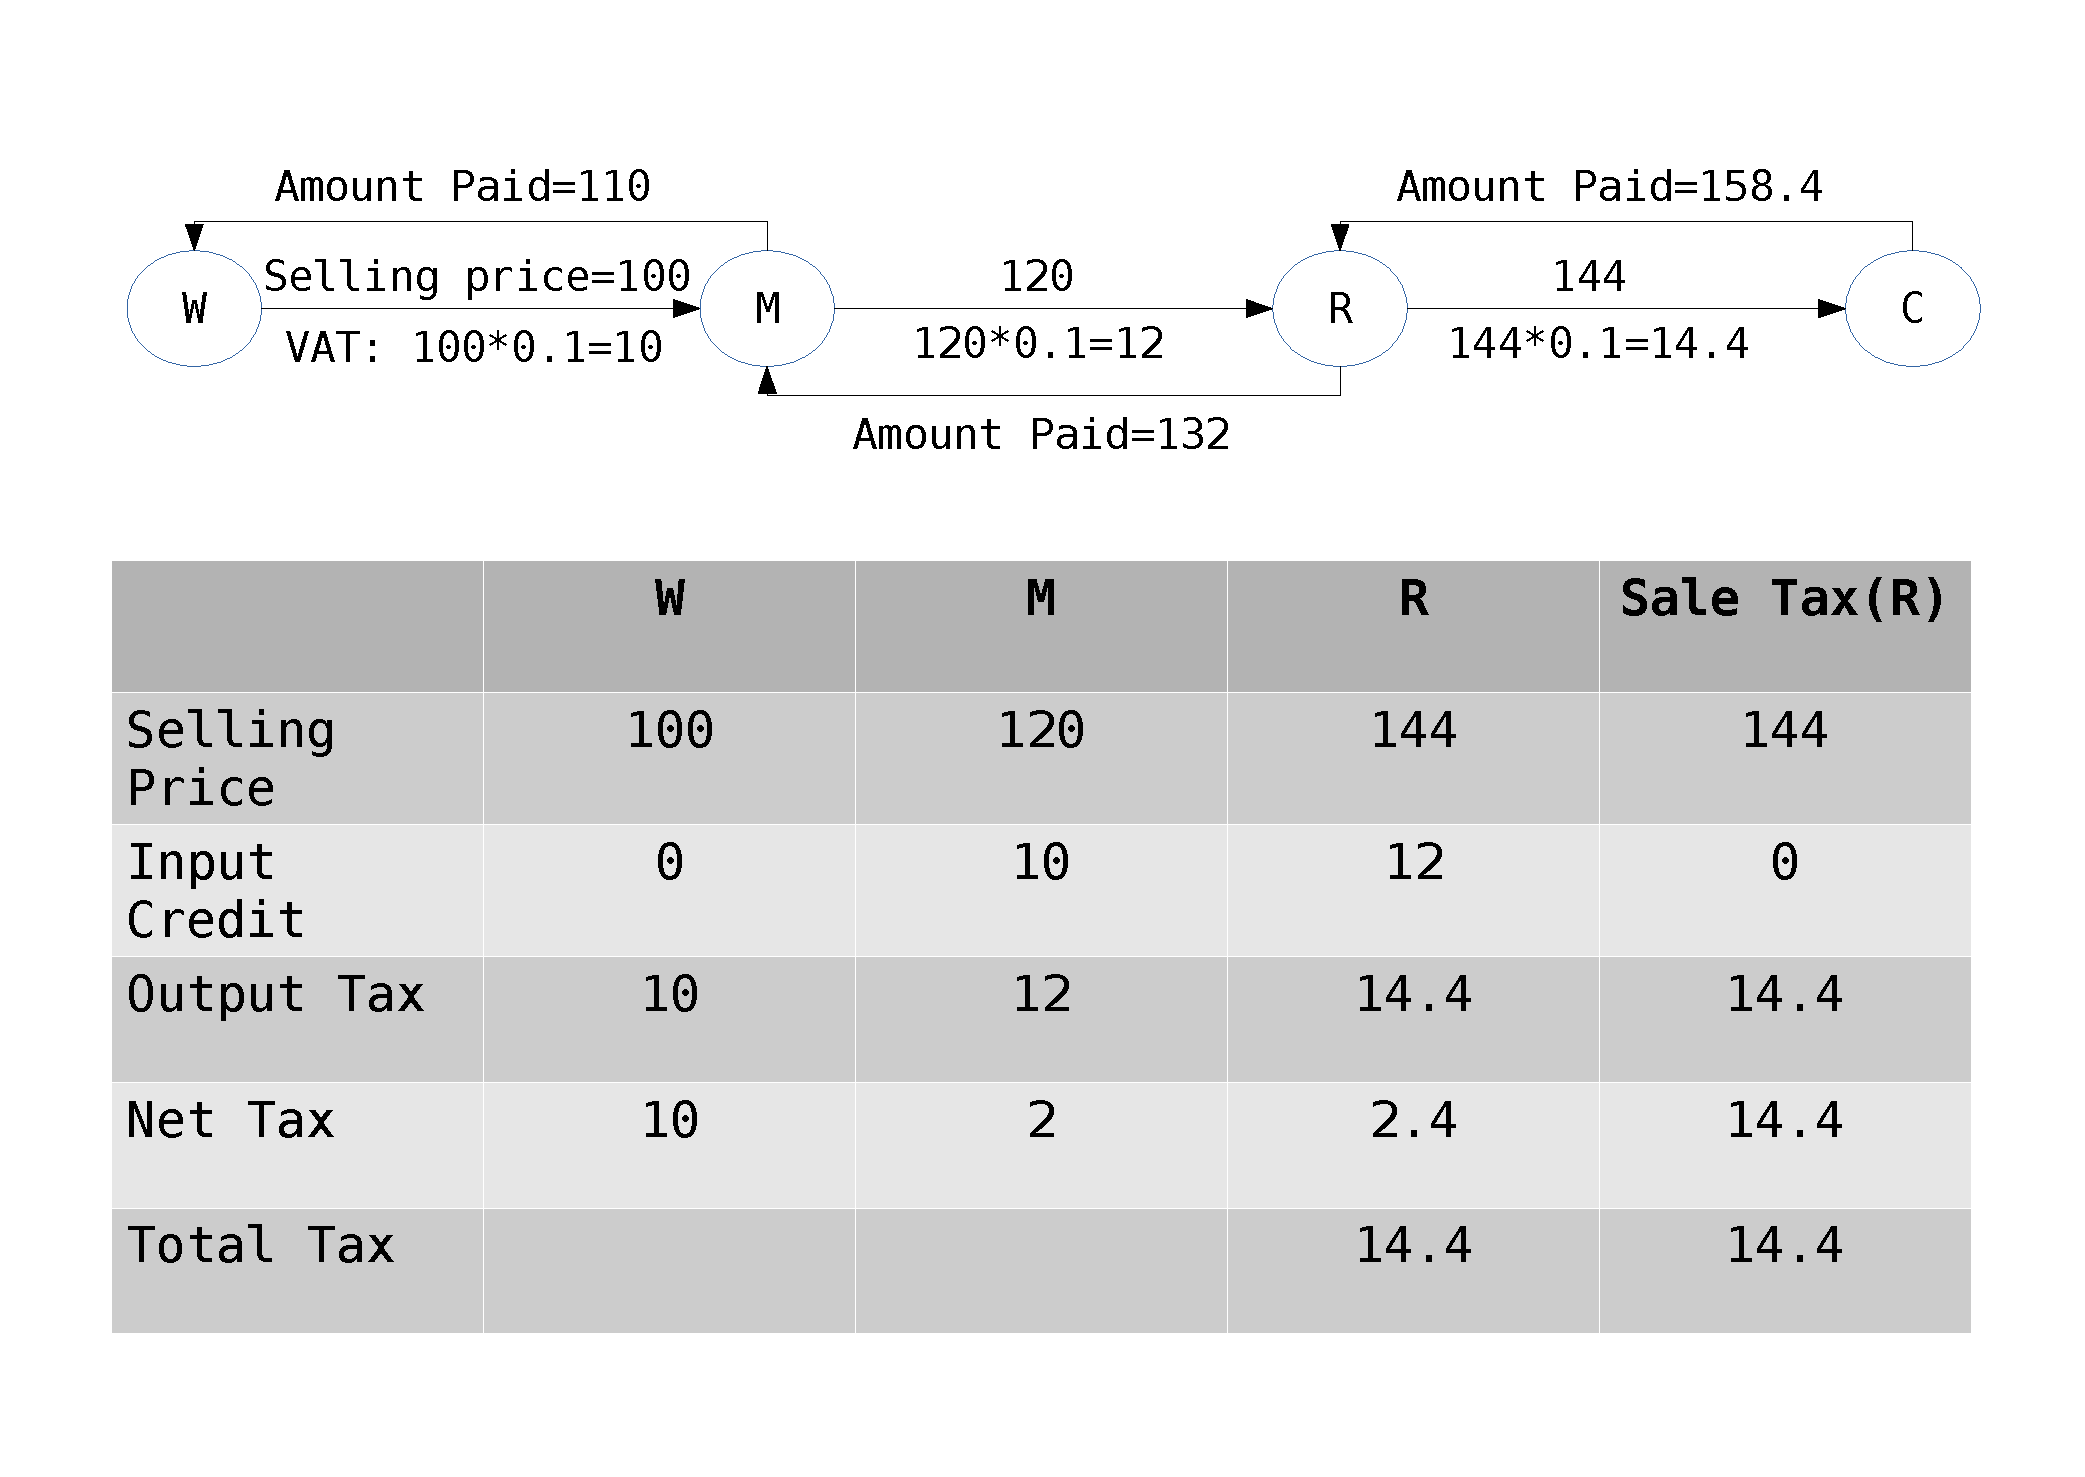
\includegraphics[width=.9\textwidth]{graphs/example_4.pdf}
\caption{Toy Model}
\label{fig:toy-model}
\floatfoot{\footnotesize An illustrative example describing how a value added tax system is different from a sales tax regime. Both the systems are revenue equivalent. In a sales tax system, the tax revenue is withheld and remitted only from the point at which sales are made to the final customer. However, in a VAT system, the tax revenue is withheld and remitted across all stages of production.}
\end{figure}

We next outline a simple example to explicate the working of the VAT to highlight features relevant for a low compliance environment. Consider a production chain as outlined in \cref{fig:toy-model} consisting of three firms and a final consumer - starting with W at the ``top'' of the chain on the left through to the final customer C at the ``end'' of the chain. Under a standard sales tax regime with ful compliance with a tax rate of 10\%, W and M do not withhold any tax. C pays \$14.4 (10\% of 144) to R as tax and R is presumed to remit the entire amount to the tax authority. Now under a
VAT regime, W withholds \$10 in tax from M (10\% of 100), M withholds \$12 in tax from R, and R will withhold \$14.4 in tax from C. Finally, W will remit \$10 to the tax authority. M, however, will declare that it has already paid \$10 as tax to M and will deduct that amount from the \$12 it withheld and will remit only \$2, and similarly, R will remit only \$2.4. The amount that should finally be deposited to the the tax authority is still \$14.4. Therefore, in a system with full compliance, the VAT system collects the same tax revenue as a standard sales tax.

There are two key points worth emphasizing here. First, M (R) gets a ``tax credit'' (also called ``input credit'') only if W (M) is registered with the tax authority. This, theoretically, should push firms which sell to registered firms to register themselves and thereby reduce informality in the system. However, in practice the effectiveness of this incentive is far from clear given the difficulties faced by developing countries in persuading firms to become formal and in monitoring the VAT system.\footnote{\cite{bird2005value}. See also \cite{DePaulaScheinkman:2010} for a model showing that such incentives can also create ``chains'' of informality.} In our study
approximately 75\% of firms make some some sales to unregistered firms.\footnote{Note we cannot distinguish between final consumers and unregistered firms in our data. However, sales to unregistered entities occur at all nodes on a VAT chain, not just at the end point.}

Second, as is standard in VAT systems, each firm has incentives to under-report sales and to over-report inputs so that a buyer and the corresponding seller have opposed incentives. For example, in the transaction between W and M, W has an incentive to not report the transaction to avoid remitting to the state any tax it has withheld while M wants to report the entire amount to maximize its tax credit. Therefore, M's incentives should act as a check on behavior of W particularly if the tax authority can credibly cross-verify M's reports with W's reports. 

If, however, M can sell to unregistered firms, then the tax authority can no longer third-party verify all of its sales. This failure of third-party verification in turn opens up the possibility of collusion between W and M.  For instance, if M sells \$ 60 worth of goods to unregistered firms (U), it can conceal this transaction completely since it cannot be verified by third-party reporting. This in turn provides M an incentive to collude with W to reduce reported purchases (so as to ensure that reported sales are not lower than reported purchases). For instance, they can agree upon a purchase amount of \$50. This reduces W's tax liability to \$5 relative to the no collusion scenario. This agreement does reduce M's input tax credit by \$5 as well. However, since M only reports half his sales, the decline in her output tax more than off-sets the decline in her input tax credit so that her overall tax liability falls (in this case by $50\%$) from \$2 to \$1.\footnote{Since M is not reporting the sale to U, it can give the tax-break to U by not collecting the tax or it can withhold the tax but not remit it. Anecdotally, we are aware of both the scenarios occurring in Delhi and we are indifferent between them.} (Refer to \cref{tbl:evasion-desc})

\begin{table}[t]
%\footnotesize
\begin{threeparttable}
\caption{Evasion in Toy Model}
\begin{tabular}{|l|l|l|l|l|l|l|l|l|c|c|}
\hline
& \multicolumn{4}{|c|}{Sales} & \multicolumn{4}{|c|}{Purchases} & \multicolumn{2}{|c|}{Tax} \\ \hline
& \multicolumn{2}{|c|}{Actual} & \multicolumn{2}{|c|}{Reported} & \multicolumn{2}{|c|}{Actual} & \multicolumn{2}{|c|}{Reported} & Actual & Reported \\ \hline
& (1) & (2) & (3) & (4) & (5) & (6) & (7) & (8) & (9) & (10) \\ \hline
& R & U & R & U & R & U & R & U & & \\ \hline
W & 100 &0 & 50 & 0 & 0 & 0 & 0 & 0 & 10&5 \\ \hline
M & 60 & 60 & 60 & 0 & 100 & 0 & 50 & 0 & 12 -10 = 2 & 6-5 = 1\\ \hline 
R & 0 & 72 & 0 & 60 & 60 & 0 & 60 & 0 & 7.2-6 = 1.2 & 6-6 = 0 \\ \hline
\end{tabular}
\begin{tablenotes}[para,flushleft]
Actual columns indicate the true values of sales or purchases. Reported columns indicate the declared values of sales or purchases. Columns (1), (3), (5), (7) show transactions with registered firms. Columns (2), (4), (6), (8) show transactions with registered firms. Tax evasion is feasible because M makes half of its sales to unregistered firms.   
\end{tablenotes}
\label{tbl:evasion-desc}
\end{threeparttable}
\end{table}


Continuing with the example as above we can consider three different scenarios depending upon whether M and R collude.  First, we assume that there is no collusion between R and M and R reports sales truth-fully. In this case, R sells output to final consumers for \$72 collecting \$7.2 in taxes of which \$6 are off-set by his input tax credit so that \$1.2 is remitted to the authority. Second, consider the case where R and M do not collude but R decides unilaterally to under-report sales to C since such sales are not subject to third-party verification. In this scenario, R can in principle report any amount of sales to C but perhaps recognizing that zero (or negative) value-added in the final step may invite further scrutiny, will report the smallest amount about \$60 he is comfortable with to the tax authority. Third, M and R have incentives to collude so that the entire transaction can be carried out without involving another party U. In particular, M and R can agree to make \$60 worth of transactions on-the-books and remaining \$60 off-the-books.

\begin{figure}[t] 
\caption{Third party verification}
\label{fig:matching_model}
%\centering
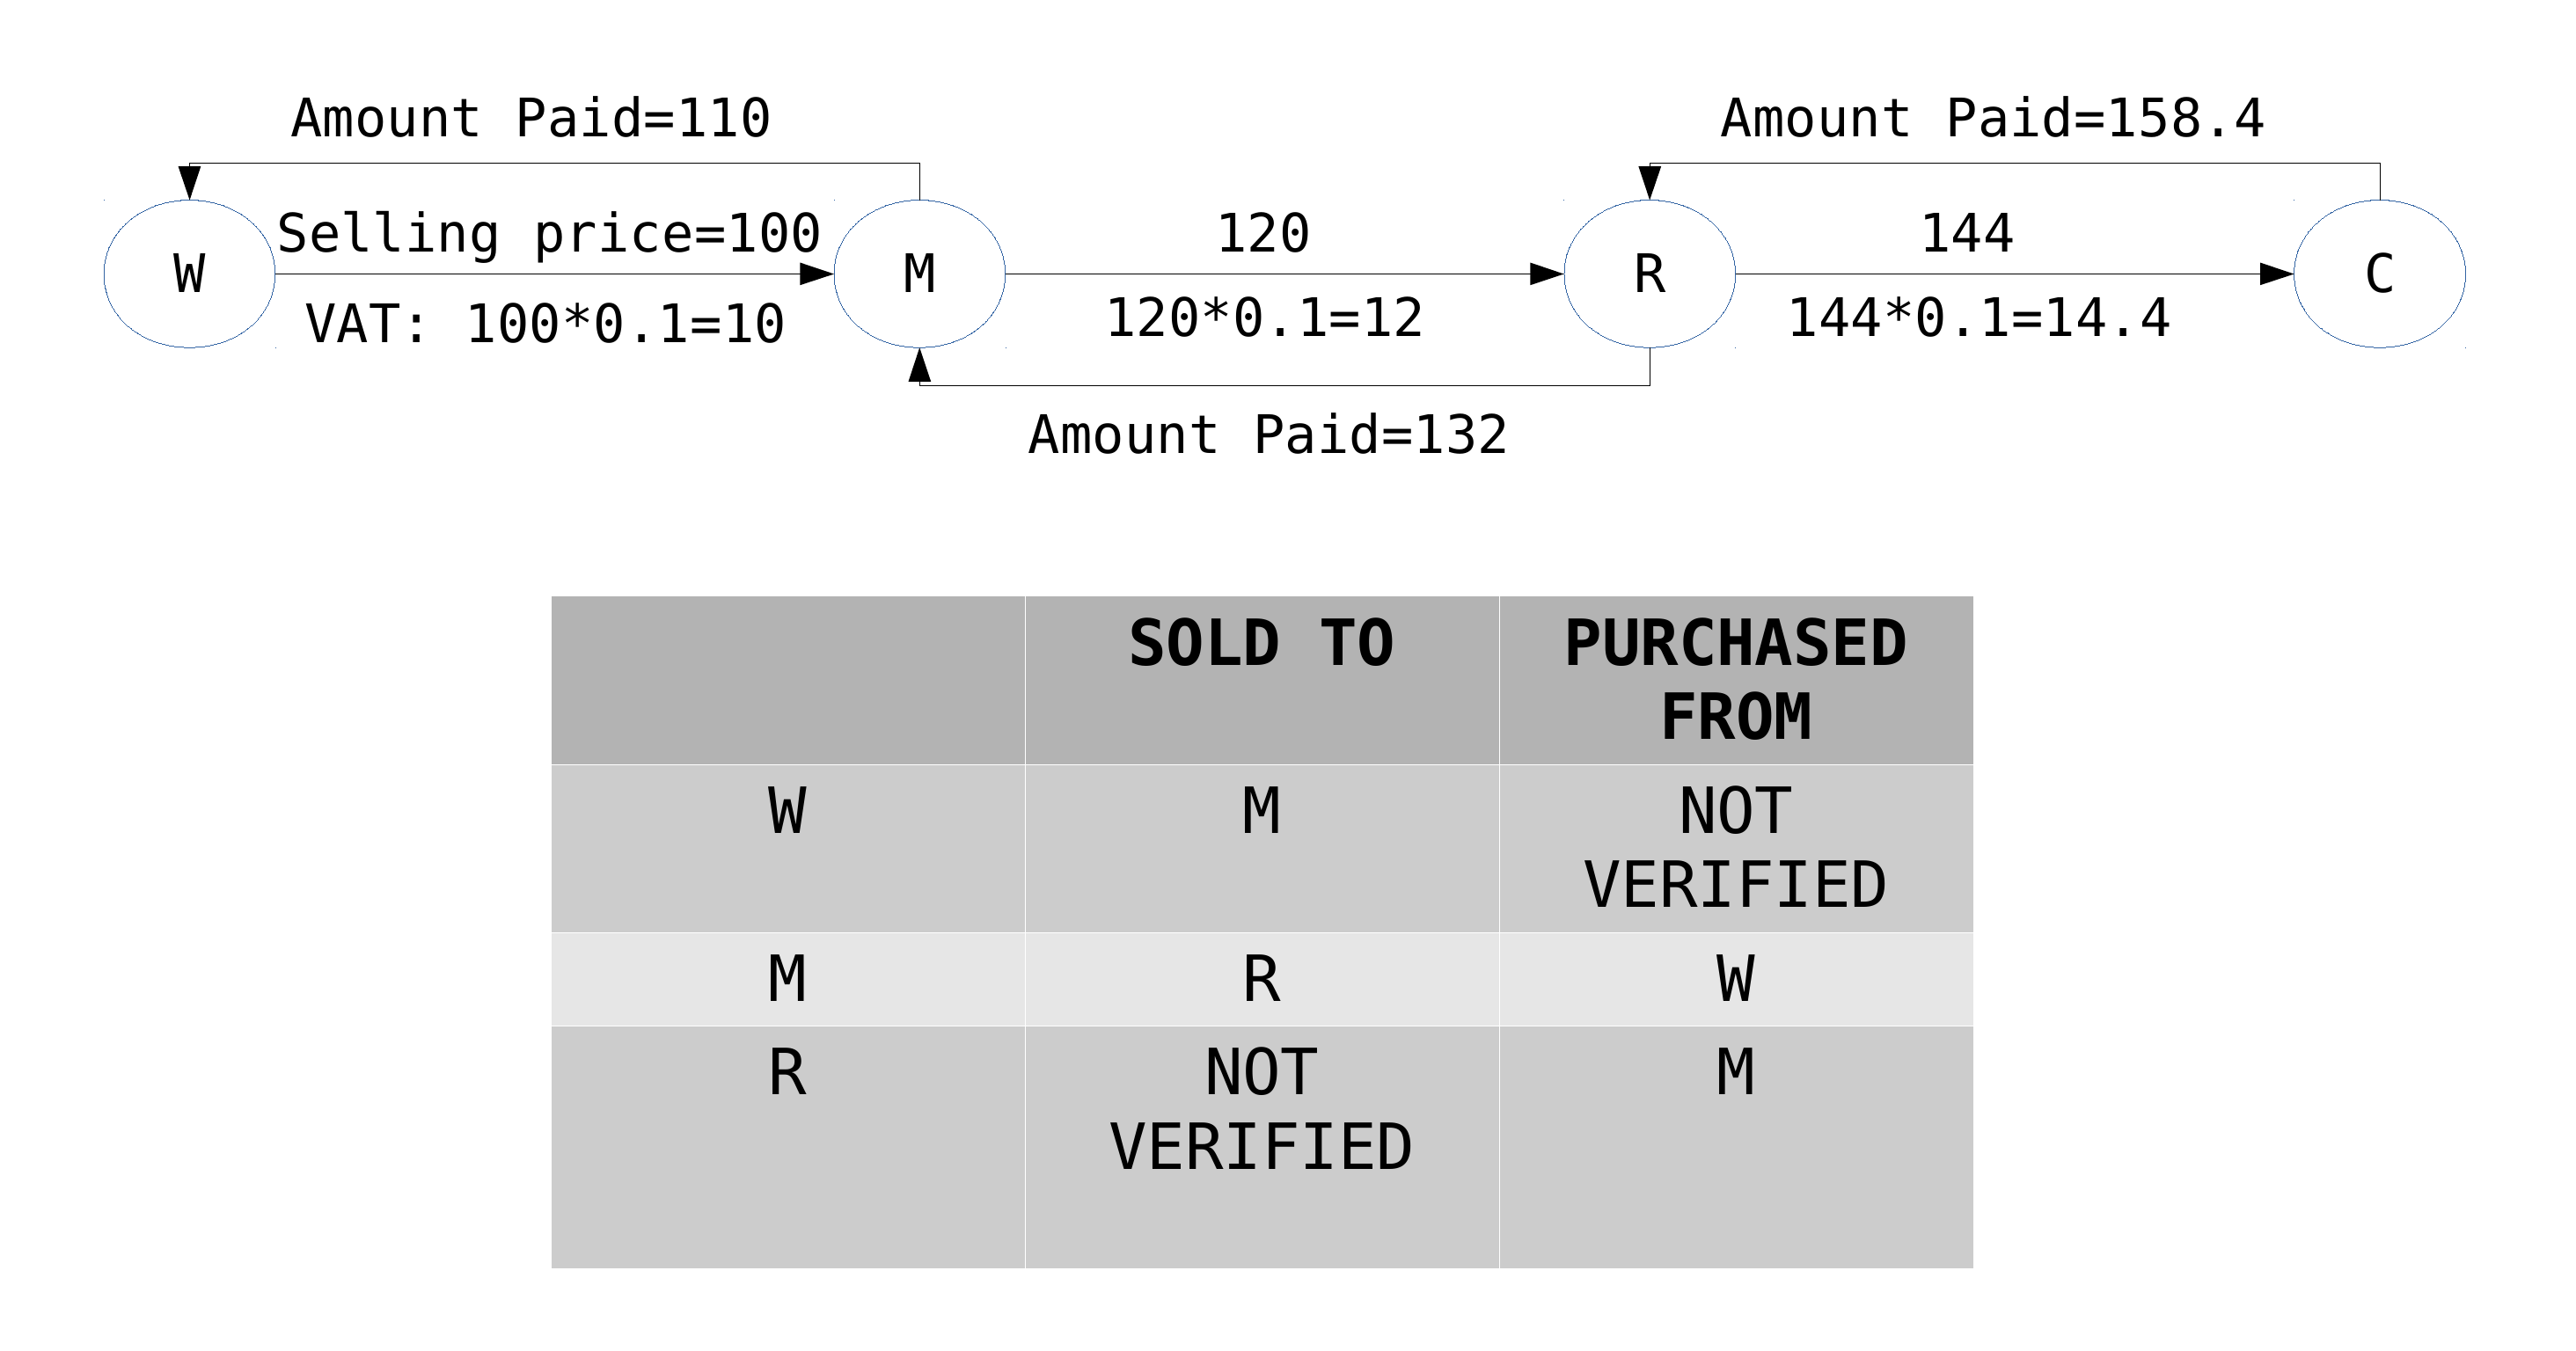
\includegraphics[width=.9\textwidth]{graphs/example_5.png}
\floatfoot{\footnotesize Description of information declared by firms. For example, W will have information about M in its SOLD TO annexure and will have no information in its PURCHASED FROM annexure. Correspondingly, M will declare information about W in its PURCHASED FROM annexure, which can be used to verify sales made by W.}
\end{figure}

The simple example above makes two points relevant for our setting. First, holding constant the probability of detection, sales to unregistered firms by a seller at any point in the chain enables pairwise collusion between the seller and his immediate supplier regardless of the presence of collusion further below (or above) the pair. This in turn implies that we can use the \cite{kleven2016can} model to analyze the implication of third-party reporting since we can limit attention to pairwise comparisons of buyers and sellers and do not need to rely on ``unraveling from the bottom'' arguments typically invoked to examine evasion in VAT systems. Second, one can reasonably interpret the pre-reform status quo within the model as the situation where no transactions had effective third-party verification and tax reports were not matched across buyers and sellers. The imposition of automated matching between buyers and sellers means that the transactions between W and M and M and R now need to be evaluated as above while the transactions between R and C are still not third-party verifiable (see \cref{fig:matching_model}). This difference across W and R firms in the effect of the policy along form the basis of our identification strategy.


\subsection{VAT in Delhi: Policy Change}
\label{background_policychange}
From Q1 of 2012-13 (year 3 of our data), firms were required to file two additional forms (known as Annexure 2A and Annexure 2B) in addition to their usual consolidated returns (which is referred to as Form 16, \cref{sec:consolidated_form}). The main change for our purposes is that the additional forms required firms to provide transaction details (i.e. sales and purchase information) disaggregated at the firm and tax-rate level for all registered firms and that the authority began to cross-check buyer and seller reports automatically on its own server.\footnote{Different commodities are taxed at different rates. Firm A reporting transactions with Firm B would group together all transactions for commodities taxed at the same rate into a single transaction report.}

Annexure 2B recorded all firm sales in the past tax period disaggregated at the registered buyer level for each tax rate. Annexure 2A recorded purchases  disaggregated at the seller level for each tax rate (refer to \cref{sec:annexure_form}). All firm level entries in Forms 2A and 2B had to include the tax IDs of all registered firms involved in the transaction thus enabling the tax authority to easily cross-check reports. The only across firm aggregation that was permissible was for unregistered firms (i.e. firms with no tax identification numbers which includes final consumers). The new forms meant that for the first time the tax authority could cross-check buyer and seller reports (for dis-aggregated transactions) from the submitted returns alone (i.e. without having to resort to an audit).\footnote{Recall that before the policy change (from 2005-2012) firms did not have to provide firm-level reports of purchases or sales but instead were only required to report total sales aggregated across all firms and correspondingly total purchases aggregated across all registered firms (and the corresponding purchase amount from unregistered firms). They were required to maintain firm-level information for their own records in case of an audit - though based on the audit notice data that we have, probability of getting audited is extremely low (less than 1\%).}

\section{Data}
\label{sec:1-data}
We have detailed tax data from the government of New Delhi for 5 years (from 2010 to 2015) which we describe in detail below.

\subsection{VAT Returns}
\label{subsec:1-data-returns}
We have anonymized VAT returns for the entire universe of registered firms for 5 years - 2010-11 (Y1), 2011-12 (Y2), 2012-13 (Y3), 2013-14 (Y4), 2014-15 (Y5). Each firm is assigned a unique identifying number so we can follow a firm over time as well as track its presence in other firms' returns (from Y3 onwards). However, anonymization implies
that we cannot link the firms to any other publicly available information on the firms.

We have detailed information on the line items in the consolidated returns (form 16) throughout the study period, and after quarter 1 of 2012-13, we have line items of form 2A and form 2B (refer to \cref{sec:consolidated_form} for details). For the purposes of this paper, we use the following information from form 16:

\begin{enumerate}
\item Total turnover (sales) disaggregated by destination - (i) local (within state) sales and (ii) inter-state or international sales. Local sales are taxable and can include sales to registered firms (which are third-party verifiable) and sales to unregistered firms (which are not third-party verifiable). However, the tax forms do not require firms to differentiate between the two. After quarter 1 of 2012-13, we can use information in form 2A and form 2B to construct our own measures to categorize the sales, but form 16 does not explicitly ask for this information.
\item Total tax withheld by the firm from local sales - this is referred to as the output tax liability. This is a tax liability and needs to be deposited with the tax authority after the requisite adjustments -- viz. the deduction of input credits, see below.
\item Total purchases disaggregated by destination - (i) local (within state) purchases and (ii) inter-state or international purchases. Local purchases are decomposed into purchases to registered firms (which are third-party verifiable) and purchases from unregistered firms (which are not third-party verifiable). Only local purchases from registered firms are eligible for input tax credits.
\todo[inline, caption={Question from AM}]{Q: Do we ever do DID on interstate outcomes? Ans: We did and no change}
\item Total tax paid by the firm on local purchases from registered  firms - this is referred to as input credit. Input credit is subtracted from the firms' output tax liability when computing the tax the firm needs to remit to the tax authority.
\item For the three post-reform years (Y3, Y4, Y5) we also have quarterly information on sales and purchases from forms 2A and 2B as described earlier (\cref{sec:annexure_form}).  For each quarter and each tax-rate, sales made by a firm are disaggregated at the (registered) firm and tax-rate level, and likewise purchases are disaggregated at the (registered) firm and tax-rate level. Therefore, for each firm, items (1)-(4) are available at the firm quarter and tax rate level.
\item Finally, the total tax remitted by the firm to the tax authority.
\end{enumerate}

Items (1)-(4) above are further broken down by tax-rates (since different goods are taxed at different rates) and we also observe some additional information such as penalties, past tax credits and liabilities. 

\subsection{Firm Characteristics}
\label{subsec:1-data-dp}
In addition to tax return information we also have basic information provided by the firm at the time of registration. We observe the date of registration, the revenue ward (i.e. the broad, largely, geographic
categorization of the firm for revenue purposes), the nature of business (e.g. manufacturer, wholesaler, retail trader, exporter, importer), the legal status of the business (e.g. proprietorship, private limited company, public sector undertaking, government corporation) as well as the other tax schemes and acts the firm is
subject to (e.g. the central excise act, service tax) and whether a firms is registered for international trade (import or export).
\todo[inline, color=green, caption={Question from AM}]{Can we use this extra information to better classify some of the retailers}

\subsection{Audit Notices}
\label{subsec:1-data-audit}
We have information (for Y4 and Y5) audit notices sent out by the tax authority. These dated notices identify the targeted firm and are usually the first step in a sometimes lengthy audit procedure. We use this information to quantify the extent to which the tax authority checks on problematic returns.

\subsection{Sample}
\label{subsec:sample}
We limit our analysis to firms present throughout the period of study. This sub-sample comprises 85\% of all firms present in year 1 and 95\% of all tax revenues in year 1. Thus, the sample consists of the near universe of revenue generating firms (see \cref{fig:vatdeposited-all} and \cref{fig:vatdeposited-alwayspresent}). We do not, therefore, address the effect of the policy on firm registration and exit decisions. We restrict our primary sub-sample further to firms that are exclusively wholesalers or retailers as reported on their VAT registration forms.\footnote{Given the previous selection rule this means we are  restricting ourselves to firms registered in or before 2010-11.} These comprise 27\% of all firms present in year 1 and 44\% of all tax revenues in year 1.\footnote{In terms of year 5, these firms comprise 19\% of the sample but still contribute 43\% of the tax revenues.} However, we use larger sub-samples for some specifications which we describe in greater detail in section \ref{sec:1-results}. In addition, we also provide additional data description in \cref{sec:overall_analysis}.

\todo[inline,caption={Firm Exit},color=green]{We Should Look at Firm Exit in our sample at Some Point.}  

\section{Empirical Strategy}
\label{sec:empirical_strategy}
We adopt a quasi-experimental approach to examine the effectiveness of the increased information available to the tax authority.

\subsection{Identification: Wholesalers vs Retailers Over Time}
\label{subsec:identification}
Relative to wholesale firms, retail firms are more likely to sell to final consumers and conversely wholesalers are more likely to sell to registered firms.\footnote{Verified in \cref{fig:salesregistered}.} As pointed out earlier, the change in filing requirements should therefore affect the two differentially. Following the reform, the tax authority can easily cross-check wholesaler sales to registered firms whereas previously this would only occur via an extensive and time-consuming audit process. On the other hand, sales made by retailers (any firm in general) to final consumers remain unaffected by the policy change. Finally, purchases by both types of firms from registered firms should be affected equally. This argument suggests then that if wholesalers find it harder to understate sales, then we should expect the policy to lead to an increase in taxes remitted by wholesalers driven by an increase in output tax declarations.\footnote{See also the discussion in \cref{sec:conceptual} which links to the relevant theoretical literature.}

Our identification strategy is thus a difference-in-difference approach comparing the difference in trends between wholesalers and retailers before and and after the policy reform. The key identifying assumptions are that the timing of the third-party verification policy introduction is exogenous for our outcomes of interest and that in the absence of the reform, the (counterfactual) evolution of outcomes among wholesalers would evolve just as the (observed) evolution of outcomes among retailers (the "parallel trends" assumption). The multiple years of data before and after the reform allows us to look at the evolution of outcomes over relatively long time periods, see \cref{sec:eventstudy-analysis}.

\subsection{Model Specification}
\label{subsec:identification_model}
The main outcome variable is the amount of VAT remitted. However, as is typical in these settings the dispersion in tax remitted is quite large (refer to \cref{fig:lorenzyear1}).\footnote{Others e.g. \citet{pomeranz2015no} finds similar dispersion for VAT returns.} Further, a large number of firms (roughly 49\%) remit zero VAT. This implies that the mean may not be a representative measure of central tendency and mean regression estimates may be sensitive to outliers. We address this concern by using alternative outcome variables and estimation methods (in addition to using standard mean regressions). Specifically, we look at linear probability model using as an outcome an indicator variable equal to one if the VAT deposited is larger than zero (for the extensive margin results). In addition, we also use quantile regressions and tobit type models (although incorporating fixed-effects for a large set of firms is a computational challenge for both methods) and also estimate linear regression models over sub-samples defined by membership in deciles of relevant firm-characteristics.

\todo[inline,caption={Need to do Quantile Regressions},color=green]{We need to implement quantile regressions with fixed effects at some point.}{ }

Our basic specification is
\begin{equation}\label{eq:basic}
y_{it}=\alpha_i+\nu_t+\beta*\text{Post}_{it}+\gamma*\text{Post}_{it}*\mathbb{I}\{\text{Wholesaler}_{i}\}+\epsilon_{it}
\end{equation}

$\text{Post}_{it}$ is equal to 1 if the observation for firm $i$ comes from the post-policy period -- years 3--5 for the annual analysis and quarters 9--20 for the quarterly analysis since the policy was introduced between years 2 and 3 and quarters 8 and 9 -- and zero otherwise. $\text{Wholesaler}_{i}$ is a dummy variable equal to 1 if firm $i$ self-reports as being a wholesaler and 0 if the firm self-reports as a retailer. The $\nu_{t}$ are a full set of time dummies and $\alpha_{i}$ are firm fixed-effects. The main outcome variables of interest are (a) an indicator for whether the firm remitted any positive amount of VAT, and (b) the amount of VAT remitted. To dig deeper into whether the effect of the policy is coming from the input side (i.e. by reducing input credits) or from the output side (i.e. by increasing the output tax liability) we
also estimate regressions using (c) input credit claimed and (d) total output tax liability as outcomes. We also construct a new outcome variable which is the difference between output tax liability and input tax credits. This allows our outcome variable to be negative and takes care of the concerns arising out of there being a mass point at
zero. All the outcome variables have been inflation adjusted to the corresponding baseline price levels i.e. outcome variables for the annual analysis have been indexed at the 2010 level, and outcome variables for the quarterly analysis have been indexed at the Q1-2010 level. 

The parameter of interest is $\gamma$ which captures the differential effect of the policy on wholesalers relative to retailers. Under the maintained "parallel-trends" assumption, for which we provide supportive evidence below, $\gamma$ is consistently estimable using standard fixed-effect methods. We also present more flexible specifications that allow for time-varying differences in group means both before and after the policy reform. In particular, we include time-dummies for each period and also interaction between each time-dummy and a wholesaler dummy. Concretely,

\begin{equation}\label{eq:flex}
y_{it}=\alpha_i+\nu_t+\gamma_t*\nu_t*\mathbb{I}\{\text{Wholesaler}_{i}\}+\epsilon_{it}
\end{equation}

Where, in addition to the firm-fixed effects $\alpha_i$ and the set of time-dummies (represented here in the interest of brevity and clarity by $\nu_t$ here), we now include a full set of time-dummies interacted with the wholesaler dummy (represented here as $\nu_t*\mathbb{I}\{\text{Wholesaler}_i\}$). The coefficients $\{\gamma_s\}_{s \in S }$\footnote{S denotes the set of post-policy time periods.} are the parameters of interest and are intended to capture the differential effect of the policy on wholesalers (relative to retailers) in period s relative to the period immediately prior to the policy's introduction. Finally, in all analysis standard errors are clustered at the firm level. In \cref{subsec:falsification-test} we present additional robustness in quarterly results by adding $\text{Pre}_{it}$ dummy which is equal to 1 for tax quarters 7 and 8 i.e. just before the introduction of the policy.

\section{Results}
\label{sec:1-results}

\subsection{Description: Wholesalers vs Retailers}	
\label{subsec:descripton_treatment_control}
Our main sample comprises of 32,979 retailers and 19,515 wholesalers who file a return during the entire period of our study.\footnote{This is when returns are aggregated to the annual level. We discuss the sample size when we consider quarterly frequency regressions in \cref{sec:quarterlyresults}.} Pre-policy means in year 1 along with changes in means over the pre-policy period for the two groups are shown in \cref{tbl:group1_summary_real}. In general, wholesalers are considerably larger than retailers; we provide additional data description in \cref{sec:overall_analysis} and discuss evidence of parallel trends in \cref{subsubsec:evidence-parallel-trends}.

\begin{table}[t]
\footnotesize  
%\scriptsize  
\begin{threeparttable}
\caption{Summary Statistics: Retailer and Wholesaler Sample (Real terms)}
\begin{tabular}{lHccHcc} \hline \hline
 &&(1)&(2)&&(3)&(4)\\
Variables & &Retailers & Diff & & Wholesalers & Diff  \\ \hline
\% Positive VAT Deposited Firms & 32979 & 0.59 & -0.00 & 19515 & 0.53 & -0.00\\
&&(0.00)&(0.00)&&(0.00)& (0.00)\\
VAT Deposited & 32979 & 0.64 & 0.02 & 19515 & 1.31 & -0.01\\
&&(0.06)&(0.02)&&(0.20)& (0.05)\\
Total Turnover & 32979 & 24.27 & 2.23 & 19515 & 80.80 & 4.70\\
&&(1.31)&(0.74)&&(6.47)& (2.59)\\
Turnover (Local) & 32979 & 18.43 & 1.89 & 19515 & 49.72 & 4.66 \\
&&(1.18)&(0.68)&&(4.45)& (1.23) \\
Credit Claimed & 32979 & 0.95 & 0.10 & 19515 & 1.41 & 0.23 \\
&&(0.04)&(0.01)&&(0.24)& (0.08)\\
Output Tax & 32979 & 1.53 & 0.12 & 19515 & 2.63 & 0.22\\
&&(0.08)&(0.02)&&(0.41)& (0.07) \\
Tax Remitted/TotalTurnover & 32028 & 0.01 & -0.00 & 18994 & 0.01 & -0.00 \\
&&(0.00)&(0.00)&&(0.00)& (0.00)\\
Credit/TotalTurnover & 32028 & 0.11 & -0.07 & 18994 & 0.07 & -0.04\\
&&(0.04)&(0.04)&&(0.03)&(0.03) \\
Output Tax/TotalTurnover & 32028 & 0.05& 0.00 & 18994 & 0.03 & 0.00\\ 
&&(0.00)&(0.00)&&(0.00)& (0.00)\\
Nonlocal Turnover/TotalTurnover & 32028 & 0.25 &0.00& 18994 & 0.37& -0.00\\ 
&&(0.00)&(0.00)&&(0.00)&(0.00) \\ \hline \hline
\end{tabular}
\begin{tablenotes}[para,flushleft]
Summary statistics for selected variables in Year 1. Amounts are in million rupees, with \rupee 65 approximately equal to \$1. $N_W=32979$, $N_R=19515$. 951 wholesalers and 521 retailers report zero turnover. Column (2) and Column (4) report mean differences between real values of  year 2 and year 1. Values have been price adjusted in year 1 terms. Standard error in parenthesis. 
\end{tablenotes}
\label{tbl:group1_summary_real}
\end{threeparttable}
\end{table}

As mentioned earlier, these two groups account for a substantial part of VAT collections. In year 1, both groups remitted 44\% (\rupee 46.7 billion) of total VAT collections and the corresponding number is 43\% for the last year of the study. In total, they account for 55.5\% of the increase in the VAT collections from the sample of firms present in each of the 5 years. \Cref{fig:group1-pretrends} and \cref{fig:group1-pretrends-quarterly} show the trends of VAT remitted at the annual as well as the quarterly level for the two groups (along with point-wise 95\% confidence intervals).


\begin{figure}[t] 
\caption{Wholesalers vs Retailers: Annual trends (in real terms) with confidence intervals}
\label{fig:group1-pretrends}
%\centering
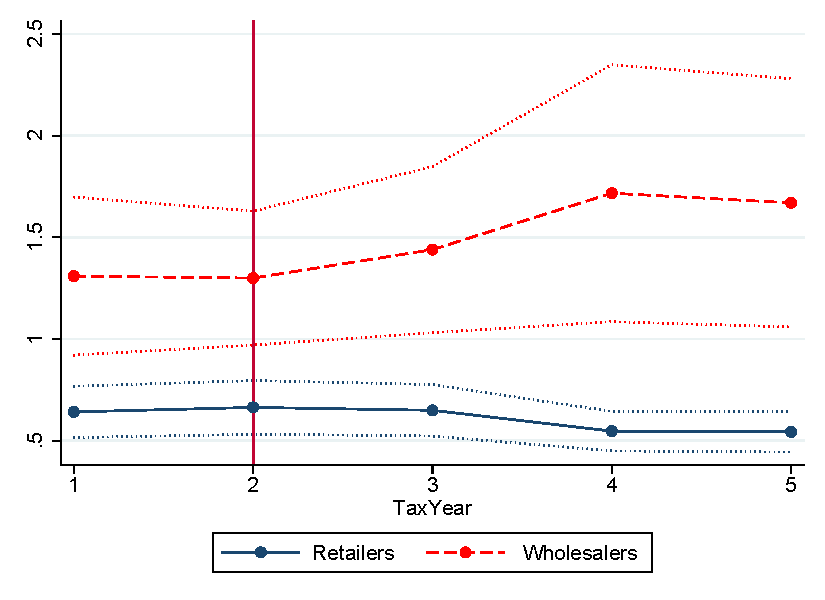
\includegraphics[width=.8\textwidth]{graphs/MeanMoneyDeposited_annual_with_confidenceintervals_Real.pdf}
\floatfoot{\footnotesize $N_W=19515, N_R=32979$. Average VAT remitted is in million rupees, inflation adjusted to 2010-11 price levels, with \rupee 65 approximately equal to \$1. Pointwise 95\% CI included. Third party verification started in year 3.}
\end{figure}


\subsubsection{Supporting Evidence for the Parallel Trends Assumption}
\label{subsubsec:evidence-parallel-trends}
We begin by providing some evidence that changes in the outcome variables of interest were evolving similarly among wholesalers and retailers in the periods prior to the reform. We  examine the key outcome variable, tax remitted by firms. \Cref{fig:group1-pretrends} presents group-wise means for tax remitted in each period and \cref{fig:eventstudy-figure-annual}(a) graphs the coefficients for the difference between the two groups in each period from estimating \cref{eq:flex}. We cannot reject the null hypothesis that the changes in tax remitted during the first two periods were the same across wholesalers and retailers (p-value=0.61). We also carry out the same analysis at the quarterly level (\Cref{fig:group1-pretrends-quarterly,fig:eventstudy-figure-quarter}(a)) which yields the same conclusions.\footnote{In \cref{subsec:eventstudy-econometrics} we describe the formal statistical tests for testing the absence of differential pre-trends in more detail.} 

This gives us some confidence that the key (untestable) assumption of parallel trends may be reasonable when examining tax remits. We also carry out the same analysis for the other outcomes of interest: (a) Output Tax, (b) Input Credit, (c) the Difference between the two and (d) whether any VAT was remitted. In all cases we cannot reject the null that the changes in outcomes in the pre-policy period were similar between the two groups.

\subsection{Results: Difference in Difference}
\label{subsec:diffindiff}
\Cref{fig:group1-pretrends,fig:eventstudy-figure-annual}(a) also suggest that wholesaler tax remits increased post-policy while retailer remits remained more or less unchanged. The regressions below formally confirm these conclusions. We begin by examining changes on the ``extensive'' margin -- changes in whether a firm remits any tax with the tax authority -- before examining changes in the amount remitted. We then examine the effect of the policy on the two key constituents of a firm's tax obligation --- input credit and output tax liability.

\Cref{tbl:group1-levels} shows the results of the difference-in-difference regressions at the firm-annual level. In column (1) the outcome is a dummy variable for whether the firm remits any tax. The proportion of wholesaler firms depositing any tax goes down by a statistically significant 2\%, though this is a relatively modest decrease of 4\% from a baseline of 53\%. Next, VAT remitted (column 2) increases by a substantively (and statistically) significant \rupee 0.38m for wholesale firms. This is an increase of 29\% over a year 1 mean of \rupee 1.31m. The wholesalers response is particularly notable since it is in start contrast to the retailer response -- for retailers total tax remitted actually decreases post-policy. These result are consistent with the conceptual framework outlined in \cref{sec:conceptual}. Wholesalers who have higher third-party verifiable income and interact with more registered firms respond much more to the improvement in third-party verification relative to retailers.

\begin{table}[t]
\footnotesize
\scalebox{0.9}{
\begin{threeparttable}
\caption{Diff-in-Diff: Wholesalers and Retailers (Annual)}
\begin{tabular}{lcHcccc} \hline
  \hline
 & (1) & (2) & (2) & (3) & (4) & (5)\\
  VARIABLES & Positive VAT  & VAT Remitted$>$ & VAT Remitted & Tax Credit & Output Tax & Output Tax -\\
   & Remitted Firms & Previous Year &  &  & & Input Credit \\ \hline
Post*Wholesaler & -0.02*** & -0.02*** & 0.38*** & -0.12 & 0.25** & 0.37*** \\
 & (0.00) & (0.01) & (0.14) & (0.15) & (0.11) & (0.14) \\
Post & 0.04*** & 0.03*** & -0.09* & 0.18*** & 0.09** & -0.09** \\
 & (0.00) & (0.00) & (0.05) & (0.05) & (0.04) & (0.05) \\\hline
Mean Dep.Var. &.53 & & 1.31 & 1.41 & 2.63& 1.22 \\
&(.00)&&(.20)&(.24)& (.41)&(0.20)\\ \hline
Observations & 262,470 & 209,976 & 262,470 & 262,470 & 262,470& 262,470\\
R-squared & 0.63 & 0.33 & 0.89 & 0.83 & 0.97 & 0.89 \\ \hline
Number of Firms & 52,494 & 52,494 & 52,494 & 52,494 & 52,494 & 52,494\\ \hline \hline
\end{tabular}
\begin{tablenotes}[para,flushleft]
Robust standard errors in parentheses, clustered at firm level. $N_W=19515,N_R=32979$. Monetary amounts are in million rupees, with \rupee 65 approximately equal to \$1. All monetary amounts have been inflation indexed to 2010-11 price levels. Column (1) shows linear probability regressions of the probability of depositing a positive amount. Column (2)-(4) respectively show regression of the mean VAT remitted by firms, input credit claimed by firms, and output tax collected by firms. To address the concern that VAT deposited has a significant mass at zero, Column(5) shows regression of the difference between output tax and input credit declared by firms.  Mean Dep. Var. shows the mean and standard errors for wholesaler firms in year 1. *** p$<$0.01, ** p$<$0.05, * p$<$0.1.
\end{tablenotes}
\label{tbl:group1-levels}
\end{threeparttable}}
\end{table}

We next examine the proximate causes of the changes in tax remitted by examining changes in output tax liability and input tax credit respectively. Consistent with the arguments in \cref{sec:conceptual} we see that there is a substantive increase in the output tax liability for wholesalers relative to retailers -- a 9.5\% increase from year one. Further, we see that input credits decline for wholesalers relative to retailers though the estimate is not significant at conventional levels. Overall, the signs of the wholesaler response along each component dimension are then consistent with the predictions of the framework outlined in \cref{sec:conceptual}. Retailer behavior is somewhat harder to rationalize. A rise in input credits is consistent with increased collusion (to minimize tax liability) or an accurate measure of purchases if under-reporting purchases is harder post-reform (recall retailers who under-report sales will have an incentive to also under-report purchases to avoid having value added estimates that are suspiciously low). We also see an increase in output tax liability for retailers post-policy and this is somewhat unexpected, particularly since retailers make most of their sales to unregistered firms. We explore this further in the next section when we examine heterogeneity in returns. Column (5) examines the difference between  output tax liability and input credits and is consistent with the argument that retailers are able to offset increases in output tax liability by matching increases in input credits (as in e.g. \cite{Carrilloetal:2017}) while wholesale firms are unable to do so.\footnote{The reason Col (5) is not the same as Col (2) is because some firms have negative tax liability and hence remit no tax.} Finally, we note that the asymmetry between effects on input credits and output tax liability suggests that that effects on wholesalers cannot be easily ascribed to a differential growth account. 
\todo[inline,caption={Comment from AM}, color=green]{What if the policy led to changes in the fraction of firms overall that were registered or unregistered. then this could just reflect fact that a firms buyers became registered post-policy}

As a robustness check, \cref{tbl:event-falsification-table} repeats the regressions whose results are presented in \cref{tbl:group1-levels} but at the quarterly frequency.\footnote{The sample is now reduced to 11,482 wholesalers and 15,337 retailers, as firms with less than \rupee 5 million in turnover only had to submit returns annually or semi-annually in the first two years of our data.} The results are consistent with the results described at the annual frequency and so we do not discuss them here. Moreover, as described earlier, we carry out event falsification test by looking at coefficients on $\text{Pre}_{it}*\mathbb{I}\{\text{Wholesaler}_{i}\}$ where $\text{Pre}_{it}$ is 1 if tax-quarter is 7 or 8 i.e. just before the introduction of the policy. We find that pre-policy effect on wholesalers is close to zero, precisely estimated, and statistically significant.\footnote{More details in \cref{subsec:falsification-test}.}

\todo[inline, caption={Question from AM}]{Don't we normalize period 8 coefficient to be zero? Ans: This is a different specification}

\begin{figure}[t] 
%\centering
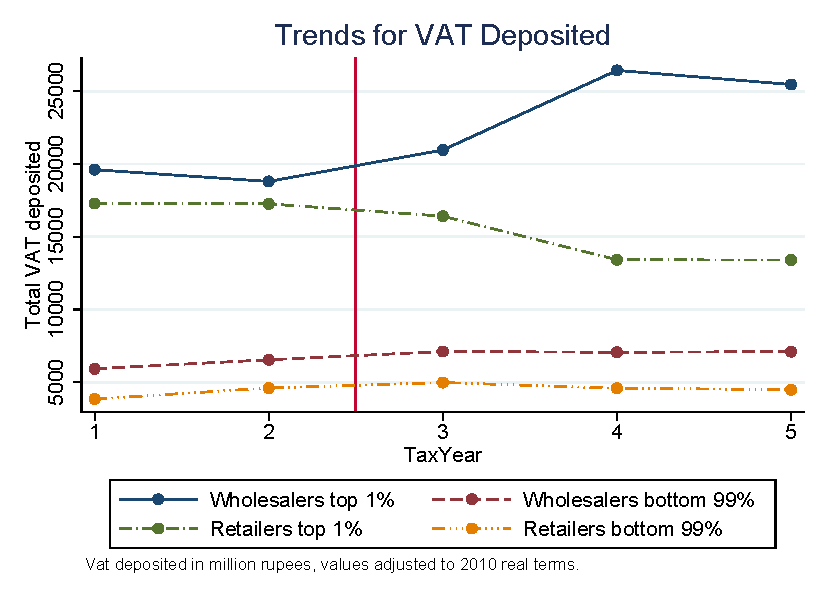
\includegraphics[width=0.8\textwidth]{graphs/MoneyDepositedTrendsTopPercentilePanel_Annual_Real.pdf}
\caption{Tax Remitted by top percentile and bottom 99\% of firms}
\label{fig:money-onepercentile}
\floatfoot{\footnotesize Notes: This figure plots the total VAT remitted by the panel of top 1\% and the bottom 99\%, in terms of VAT remitted in year 1, of wholesalers and retailers. $N_W=19515,N_R=32979$. Therefore, top 1\% of retailers are 329 firms and top 1\% of wholesalers are 195 firms. Rest of the firms form bottom 99\%. Monetary amounts are in million rupees, inflation adjusted to 2010-11 price levels, with \rupee 65 approximately equal to \$1.}
\end{figure}

\subsubsection{Heterogeneity}
\label{subsubsec:diffindiff_heterogeneity}
We next turn to exploring heterogeneity in our estimates. There are two main reasons for this. First, as we saw in the previous table, there is a significant point mass at zero for tax remitted. This suggests that exploring alternatives to mean regressions may be a useful exercise. Further, \cref{tbl:group1-levels} indicates that while the policy had limited extensive margin effects (i.e. on whether firms remit any tax) there were substantive intensive margin effects, suggesting the the policy may have affected different wholesalers differently.


\begin{table}[t]
\footnotesize
\scalebox{0.9}{
\begin{threeparttable}
\caption{Diff-in-Diff: Wholesalers and Retailers (Annual, Real Terms, Top Percentile)}
\begin{tabular}{llHllll} \hline
  \hline
 & (1) & (2) & (2) & (3) & (4) & (5)\\
  VARIABLES & Positive VAT  & VAT Remitted$>$ & VAT Remitted & Input Credit & Output Tax & Output Tax -\\
   & Remitted Firms & Previous Year &  &  & & Input Credit \\ \hline
Post*Wholesaler & 0.02* & 0.06 & 34.75** & -15.94 & 19.96** & 35.90** \\
 & (0.01) & (0.06) & (13.62) & (13.38) & (8.89) & (14.06) \\
Post & -0.02** & -0.07* & -12.02** & 9.31** & -3.47 & -12.78*** \\
& (0.01) & (0.04) & (4.68) & (4.07) & (3.65) & (4.46) \\ \hline
Mean Dep.Var. &1 & & 100.59 & 36.27 & 138.29& 102.02 \\
&(0.00)&&(18.55)&(23.42)& (39.17)&(18.39)\\ \hline
Observations & 2,620 & 2,096 & 2,620 & 2,620 & 2,620 & 2,620 \\
R-squared & 0.42 & 0.38 & 0.88 & 0.84 & 0.98 & 0.88 \\
Number of Firms & 524 & 524 & 524 & 524 & 524 & 524\\ \hline \hline
\end{tabular}
\begin{tablenotes}[para,flushleft]
Robust standard errors in parentheses, clustered at firm level. $N_W=195,N_R=329$. Monetary amounts are in million rupees, inflation adjusted to annual 2010-11 price levels, with \rupee 65 approximately equal to \$1. Column (1) shows linear probability regressions of the probability of remitting a positive amount. Column (2)-(4) respectively show regression of the mean VAT remitted by firms, input tax credit claimed by firms, and output tax collected by firms. To address the concern that VAT remitted has a significant mass at zero, Column(5) shows regression of the difference between output tax and input credit declared by firms.  Mean Dep. Var. shows the mean and standard errors for top 1\% wholesaler firms in year 1. *** p$<$0.01, ** p$<$0.05, * p$<$0.1
\end{tablenotes}
\label{tbl:group1-toppercentile}
\end{threeparttable}}
\end{table}

We begin by examining the evolution of tax remitted for different sub-groups of wholesalers and retailers. In particular, we partition each group into two sub-groups ranked according to tax remitted in the first year of the study -- the top 1\% and the remaining 99\%.\footnote{We use tax remitted as the stratifying variable because it is also the variable used by the authority to determine firms that will be examined by the special ward in charge of large tax-payers.} The results are graphed in \cref{fig:money-onepercentile}; two points are worth noting. First, tax remits remain relatively stable for the bottom 99\% of wholesale firms as compared to the top 1\%. In contrast, tax remits for retail firms as a whole (both in the 1\% as well as in the 99\% sub-groups) are relatively stable throughout the study period. This analysis suggests that it is worthwhile to examine heterogeneity in treatment effects across different percentiles of the baseline outcome distribution.\footnote{A natural estimation method here would be to use quantile regressions. We are currently working on implementing a stable quantile regression model with fixed effects on our data.} In \cref{tbl:group1-toppercentile,tbl:group1-bottom99} we present the regression adjusted comparisons of \cref{fig:money-onepercentile}. There are at least three points of interest. First, the policy has no differential effects on wholesalers relative to retailers in the bottom 99\% sub-sample. Second, the response of the top 1\% of wholesalers is sharply different from that of the top retailers. For the top retailers, input credits increase and output tax declines modestly\footnote{The output tax response is not statistically significant at conventional levels.} so that overall tax remits fall by $22.9\%$ (relative to a top 1\% retailer baseline of \rupee 52.55m) after the policy. In stark contrast, input credits decline and output tax liability increases for wholesalers (relative to top retailers) so that post-policy overall tax deposited rises by $34\%$ (relative to the baseline mean).

\begin{table}[t]
\footnotesize
\scalebox{0.9}{
\begin{threeparttable}
\caption{Diff-in-Diff: Wholesalers and Retailers (Annual, Real Terms, Bottom 99 Percentile)}
\begin{tabular}{llHllll} \hline
  \hline
 & (1) & (2) & (2) & (3) & (4) & (5)\\
  VARIABLES & Positive VAT  & VAT Remitted$>$ & VAT Remitted & Input Credit & Output Tax & Output Tax -\\
   & Remitted Firms & Previous Year &  &  & & Input Credit \\ \hline
Post*Wholesaler & -0.02*** & -0.02*** & 0.03 & 0.04 & 0.05 & 0.02 \\
 & (0.00) & (0.01) & (0.03) & (0.06) & (0.07) & (0.02) \\
Post & 0.04*** & 0.03*** & 0.03*** & 0.09*** & 0.13*** & 0.03*** \\
 & (0.00) & (0.00) & (0.01) & (0.02) & (0.02) & (0.01) \\
\hline
Mean Dep.Var. &0.53 & & 0.31 & 1.06 & 1.26& 0.20 \\
&(0.00)&&(0.01)&(0.06)& (0.06)&(0.02)\\ \hline
Observations & 259,850 & 207,880 & 259,850 & 259,850 & 259,850 & 259,850 \\
R-squared & 0.63 & 0.33 & 0.58 & 0.78 & 0.78 & 0.82 \\
Number of Firms & 51,970 & 51,970 & 51,970 & 51,970 & 51,970 & 51,970\\ \hline \hline
\end{tabular}
\begin{tablenotes}[para,flushleft]
Robust standard errors in parentheses, clustered at firm level. $N_W=19,320,N_R=32,650$. Monetary amounts are in million rupees, inflation  adjusted to 2010-11 price levels, with \rupee 65 approximately equal to \$1. Column (1) shows linear probability regressions of the probability of remitting a positive amount. Column (2)-(4) respectively show regression of the mean VAT remitted by firms, input tax credit claimed by firms, and output tax collected by firms. To address the concern that VAT remitted has a significant mass at zero, Column(5) shows regression of the difference between output tax and input credit declared by firms.  Mean Dep. Var. shows the mean and standard errors for wholesaler firms in year 1. *** p$<$0.01, ** p$<$0.05, * p$<$0.1
\end{tablenotes}
\label{tbl:group1-bottom99}
\end{threeparttable}}
\end{table}

\begin{figure}[t!] 
%\centering
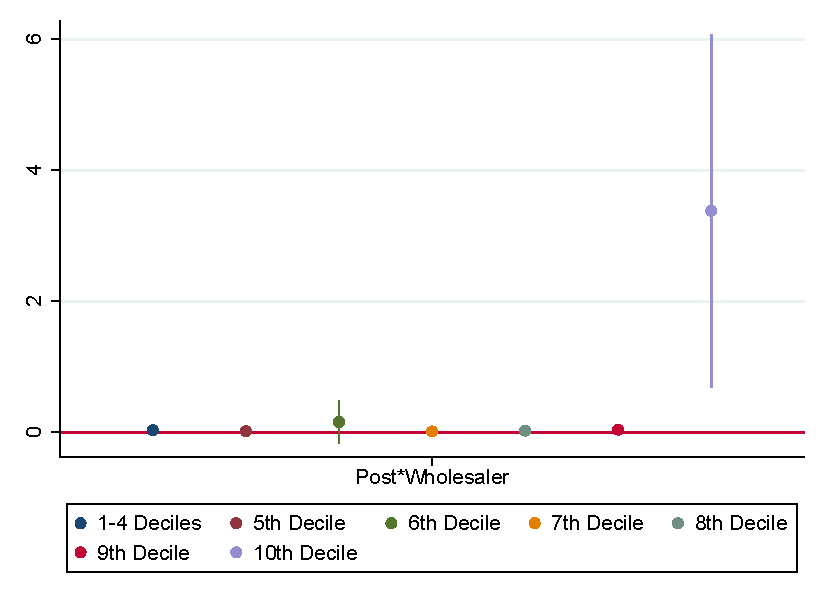
\includegraphics[width=.8\textwidth]{graphs/HeterogeneityMoneyDeposited_Real.pdf}
\floatfoot{\footnotesize Notes: This figure plots the difference between wholesalers and retailers for different deciles, based on VAT remitted in the first year. The x axis indicates the decile. Confidence intervals at the 95\% level. $N_W=32979$,$N_R=19515$. Coefficients are in million rupees, inflation adjusted to 2010-11 price levels, with \rupee 65 approximately equal to \$1.The first group consists of 4 deciles because all the firms in that group do not remit any VAT.}
\caption{Heterogeneity Analysis: VAT Remitted for Wholesalers vs Retailers}
\label{fig:heterogeneity-figure-annual-vatdeposited}
\end{figure}
These results confirm the differential effects of the policy and also help us better understand firm responses. First, the opposing signs and differences in magnitudes and significance of the output tax response between top wholesalers and retailers is consistent with the hypothesis that top wholesalers are more constrained in their responses.\footnote{As pointed out earlier a differential growth story for top wholesalers is less plausible since input credit and output tax respond in opposite directions while increased growth via sales would be more likely to be reflected in increased purchases as well.} Further, top wholesalers are both more likely to be monitored by a special tax assessment unit and have more third-party verifiable income. In contrast, top retailers are less likely to be monitored by the special unit and also have much less third-party verifiable income. The lack of any differential response among the bottom 99\% of wholesalers (relative to retailers) in turn suggests that differences in third-party verifiable income alone (without commensurate monitoring) are not sufficient for generating greater collections. These
differential effects therefore provide some sobering evidence on the effectiveness of the VAT at increasing collections in low compliance environments.\footnote{\cite{almunia2017analysis} find substantial discrepancies in third-party reports in Uganda and also emphasize the limited enforcement capacity of the state as an important constraint. In our context, discrepancies are less of a concern post-policy, because of automatic matching, relative to collusion.} Second, retailers (both large and small) increase input credits claimed after the policy while the wholesaler response is either much more muted or even negative. These results are consistent with the retailers relatively higher ability to collude with a smaller number of input supplies.
%Further, less than 5\% of the bottom 99\% of wholesalers (and $\textbf{??}$ of the bottom 99\% of retailers) are monitored by the special assessment unit.
 %(on average retailers in our sample purchased from \textbf{??} registered firms while the corresponding figure is \textbf{??} for wholesale firms)

\todo[inline,caption={SM: Numbers Needed}]{We need some numbers for the two paragrahps above. the sentences have been commented out for now. DO NOT DELETE. I am also not sure how many registered firms our wholesalers purchase from. It is not clear that this point above even makes any sense unless the numbers line up as predicted.}

\todo[inline,caption={Shekhar Size Definition Question},color=green]{SM: I though we defined size by turnover in the baseline year. That seems to be the most acceptable definition no? Also, can we check that the footnote where we use turnover gives us similar results. I know we looked at it at some point.}

\begin{figure}[t!] 
%\centering
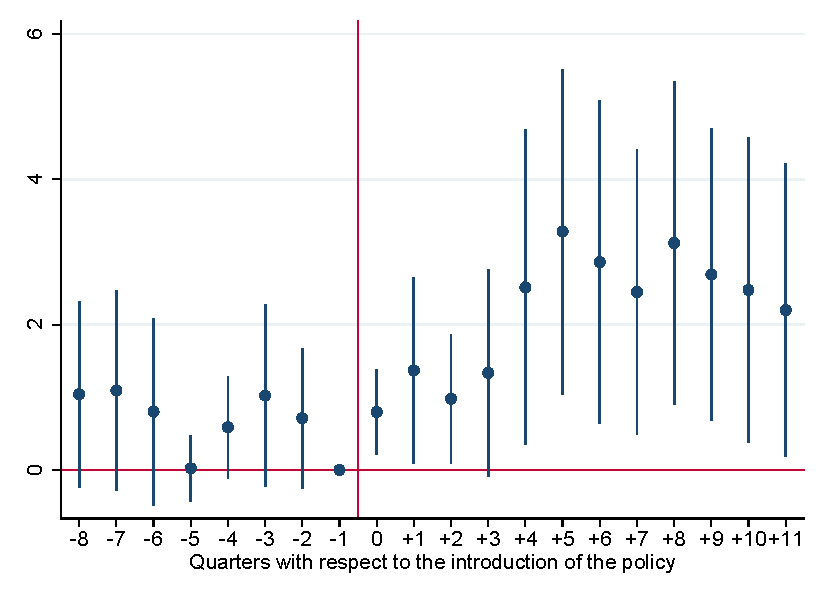
\includegraphics[width=.8\textwidth]{graphs/EventStudy-MoneyDeposited-Quarter_TopDecile_Real.pdf}
\floatfoot{\footnotesize Notes: Graphical event-study analysis of the effect of third party verification policy on wholesalers compared to retailers. Limiting the set of wholesalers and retailers to the top 10\% of each group in terms of VAT remitted in quarter 1. Confidence intervals were constructed with heteroskedasticity-robust standard errors, clustered at the firm level. The coefficient for the wholesale group in the quarter (-1) prior the policy is normalized to zero. The regressions include firm fixed  effects and time effects. The x axis indicates time, with quarterly observations and zero indicates the first year of the third party verification policy. We have 20 quarters of data from 2010-11 to  2014-15. Confidence intervals at the 95\% level. $N_W=1148$,$N_R=1533$. Coefficients are in million rupees, with inflation adjusted to Q1 2010-11 price levels, with \rupee 65 approximately equal to \$1. Pretrends are not statistically significant.}
\caption{Top Decile: VAT Remitted for Wholesalers vs Retailers}
\label{fig:eventstudy-figure-quarter-vatdeposited-topdecile}
\end{figure}

As an alternative approach we estimate \cref{eq:basic} separately for different deciles based on the baseline (year one) distribution of tax remitted.\footnote{We constructed deciles using group-specific distributions of tax remitted in year one.} \Cref{fig:heterogeneity-figure-annual-vatdeposited} plots the coefficient of interest ($\gamma$ from eq. \ref{eq:basic}) from each of the seven separate regressions though we present regression results only from the regressions using the top decile subsample in \cref{tbl:group1-decile}.\footnote{The remaining regression results are omitted for brevity and are available upon request.} \Cref{fig:eventstudy-figure-quarter-vatdeposited-topdecile} shows the event-study plots for the top decile of wholesalers and retailers on VAT remitted as an outcome variable. Other outcome variables are shown in \cref{fig:eventstudy-figure-quarter-topdecile}.

The figures and table are consistent with the earlier graph. The treatment effect is only substantively significant for the top decile, and is relatively negligible for all other deciles. Tax remitted by wholesalers in the top decile goes up by \rupee 3.38m, a 26.7\% increase over the \rupee 12.6m remitted in year one. Given the relative stability of retailer outcomes across deciles, the results imply that it is only the biggest wholesalers that are driving the large increase in tax remitted in the mean regressions in \cref{tbl:group1-levels}.

There are at least two possible reasons for the differential effects on the largest wholesalers. First, 96\% of the top 1\% of wholesalers in our sub-sample are assessed by a special tax unit (known as the Key Customers Services Unit) that is tasked with collections form large firms (the corresponding figure for the top 1\% of retailers is 80\%) and which has greater resources for inspection and other activities.\footnote{See \cite{DasGuptaetal:2004} for a discussion of similar units in the context of personal income tax in India.} Second, as we show below, the ease of third-party verification had a much larger effect on the top 1\% of wholesalers (relative to other wholesalers and retailers) since the bulk of their sales were to other registered firms. The combination of these two factors is consistent with the results in the table above. We are currently seeking more information on the special ward assigned for larger firms.

\todo[inline, caption={Do better analysis on KCS}, color=green]{Revenue and administrative efficacy of KCS. Do whatever you can think of.}

\begin{table}[t!]
\footnotesize
\begin{threeparttable}
\caption{Diff-in-Diff for Top Decile: Wholesalers and Retailers (Annual, Real Terms)}
\begin{tabular}{lcHcccc} \hline \hline
  & (1) & (2) & (2) & (3) & (4) & (5) \\
 VARIABLES & Positive VAT  & VAT Remitted$>$ & VAT Deposited & Tax Credit & Output Tax & Output Tax -\\
 & Remitted Firms & Previous Year &  &  & & Input Credit \\ \hline
 Post*Wholesaler & 0.02*** & 0.04** & 3.38** & -1.77 & 1.68 & 3.46** \\
 & (0.01) & (0.02) & (1.38) & (1.43) & (1.04) & (1.42) \\
Post & -0.06*** & 0.01 & -1.11** & 1.00** & -0.21 & -1.20*** \\
 & (0.00) & (0.01) & (0.47) & (0.42) & (0.39) & (0.45) \\ \hline
Mean Dep.Var. &1 & & 12.65 & 6.98 & 19.73& 12.75  \\
&(.00)&&(1.97)&(2.40)& (4.04)&(1.95) \\ \hline
Observations & 26,240 & 20,992 & 26,240 & 26,240 & 26,240 & 26,240 \\
R-squared & 0.41 & 0.28 & 0.89 & 0.84 & 0.97 & 0.89 \\
Number of Firms & 5,248 & 5,248 & 5,248 & 5,248 & 5,248 & 5,248 \\ \hline \hline
\end{tabular}
\begin{tablenotes}[para,flushleft]
\Cref{eq:basic} results of the effect of third party verification policy on wholesalers compared to retailers. Limiting the set of wholesalers and retailers to the top 10\% of each group in terms of VAT remitted in year 1. Robust standard errors in parentheses, clustered at firm level. Number of wholesalers is 1951 and number of retailers is 3297. Monetary amounts are in million rupees, inflation adjusted to 2010-11 price levels, with \rupee 65 approximately equal to \$1. Column (1) shows linear probability regressions of the probability of remitting a positive amount of VAT. Column (2)-(4) respectively show regression of the mean VAT remitted by firms, of the input tax credit claimed by firms, and the output tax collected by firms. *** p$<$0.01, ** p$<$0.05, * p$<$0.1.
\end{tablenotes}
\label{tbl:group1-decile}
\end{threeparttable}
\end{table}

\section{Mechanism}\label{sec:1-mechanism}
% \citet{dufloplumber} in her 2017 Ely lecture at the AEA has highlighted the importance of economists getting into the plumbing details of a policy. In this section we show some evidence which sheds light on how the policy was actually executed on the ground. 
% ;
\begin{figure}[t!] 
%\centering
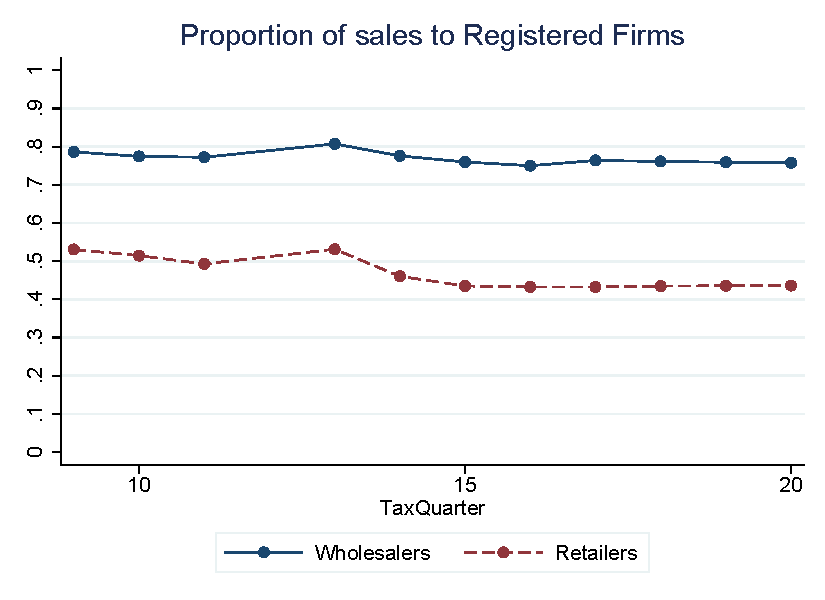
\includegraphics{graphs/ProportionSalesRegistered.pdf}
\caption{Sales to registered firms}
\floatfoot{\footnotesize Proportion of total sales made to registered firms for wholesale and retail firms.}
\label{fig:salesregistered}
\end{figure}

In this section we explore potential mechanisms for the reduced form results above. Specifically, we examine the pattern of sales made to registered firms and how it evolved over time. This is important because the conceptual framework outlined in \cref{sec:conceptual} highlighted the role of third-party verifiable transactions as a moving force and in our context only interactions with registered firms are third-party verifiable.\footnote{We explore other a few other implementation details that shed light on how the policy was actually executed on the ground in \cref{sec:execution}.}

%We begin by examining the pattern of sales made to registered firms and how it evolved over time
\subsection{Sales to Registered Firms}
\label{subsec:registered_sales}
\Cref{fig:salesregistered} displays quarterly sales to registered firms as a proportion of total sales separately for wholesalers and retailers. The graph is only from quarter 9 (year 3) onwards because in the pre-policy period firms were only required to report a total sales amount without further disaggregation. The lack of a complete series on this variable also limits its use as a direct measure of formality which could be used to examine heterogeneity (although we do present some suggestive evidence below). In addition, changes along the extensive margin for interacting firms also complicates the interpretation (e.g. if the policy led to more firms becoming registered). Over the entire post-policy period wholesale firms made approximately 78\% of their sales to registered firms while the corresponding figure for retail firms is 43\%.

\begin{figure}[t!] 
%\centering
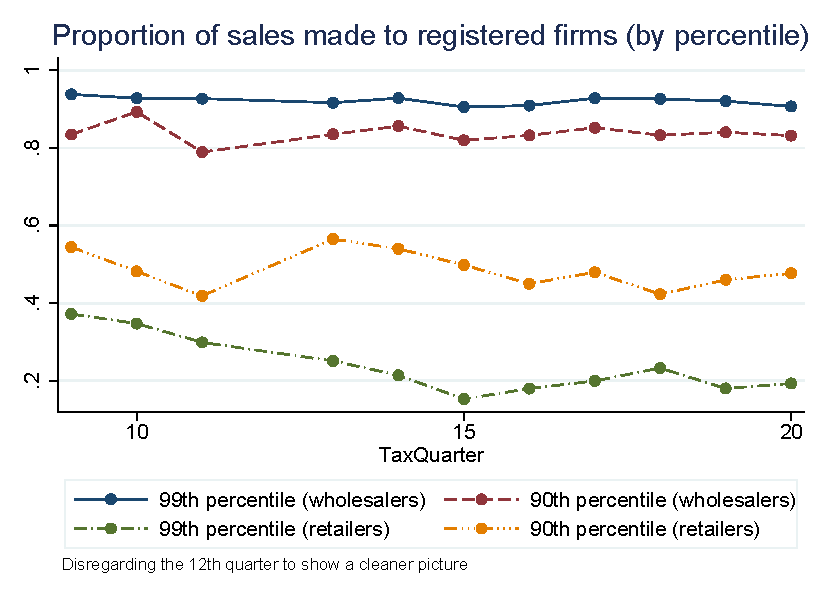
\includegraphics{graphs/ProportionSalesRegisteredTopPercentile_v2_without12.pdf}
\caption{Sales to registered firms}
\floatfoot{\footnotesize Describing the proportion of sales made to registered firms. Comparing the declarations by top percentile of wholesalers and retailers with the 90th percentile.}
\label{fig:sales_registered_percentile}
\end{figure}

We next examine this proportion for the $99^{th}$ and $90^{th}$ percentile for each group in \cref{fig:sales_registered_percentile}. There are three points worth noting: First, over 90\% of total sales are made to registered firms by the top percentile of wholesale firms (and the figure is similar, though somewhat lower for the $90^{th}$ percentile). Second, a significant proportion of sales by exclusively retail firms are made to registered firms. This is \emph{prima facie} surprising and we discuss its interpretation below. Finally, the proportion of total sales made to registered firms is lower ($\approx 20\%$) among the top percentile of retail firms compared to the $90^{th}$ percentile ($\approx 50\%$), suggesting that smaller retailers are more likely to sell to registered firms.


There are at least four potential reasons for the retailer related findings. First, a larger retailer may in turn sell to smaller (registered) retailers. This could explain the results for the top percentile of retailers but would not suffice for explaining why smaller retailers make \emph{more} sales to registered firms than
larger retailers.

A second possibility is that at least some of the reported sales to registered firms by retailers are in fact fraudulent -- that they are created to provide fraudulent input credits and hence reduce tax collections.\footnote{A simple example is the following: retailer A declares a proportion of her sales to final customers as in fact having been made to firm B. Firm A's tax obligation does not change relative to the counter-factual where all sales are reported as sales to final customers. On the other hand, Firm B reduces his tax liability so that, after accounting for the probability of detection, there is an incentive for both parties to conclude the transaction and for B to make a side payment to A.} We are exploring this possibility in ongoing work and in particular using network analysis to examine further the characteristics of registered firms who make purchases from small retailers.

%\textbf{Another simple explanation could be that retailers indeed avoid declaring a significant portion of their sales to final customers and as a result the declared proportion of sales to registered firms increases mechanically. Lastly, we should not rule out that selling significantly to registered firms is a feature of retailers as well and this is the first time we have had empirical evidence to discuss it.}

A third explanation is that greater under-reporting of sales to unregistered firms by smaller retailers (relative to larger retailers) leads mechanically to smaller retailers reporting a higher fraction of sales to registered firms relative to larger retailers. Finally, the data may be an accurate record of retailer behavior rather than a reflection of any evasion. At the moment
we do not have enough information to distinguish between these competing explanations though we are pursuing further work here as well.

We directly examine the relationship between the proportion of sales to registered firms and the change in tax collections as a result of the policy change. We conduct a triple-difference comparison by comparing the difference between wholesalers and retailers with a higher fraction of sales to registered firms to the corresponding difference between firms with a lower fraction of sales and finally doing these comparisons before and after the policy reform for the the third difference. Specifically,
\begin{multline}\label{eq:ddd}
y_{it}=\alpha_i+\nu_t+\beta*\text{Post}_{it}+
\delta*\text{Post}_{it}*\text{PropRegistered}_i\\+ \gamma*\text{Post}_{it}*\mathbb{I}\{\text{Wholesaler}_{i}\}+\lambda*\text{Post}_{it}*\mathbb{I}\{\text{Wholesaler}_{i}\}*\text{PropRegistered}_i+\epsilon_{it}
\end{multline}

In \cref{eq:ddd}, in addition to what we have already described for \cref{eq:basic}, we now also add a variable called $\text{PropRegistered}_i$ which is the proportion of sales declared to be made in quarter 9 (the first quarter immediately after the introduction of the policy). Now the coefficient of interest is $\lambda$ which tells us the effect of the policy on wholesaler firms which make greater proportion of their sales to registered firms. Another coefficient of interest is $\delta$ which shows the effect on retailers. 

\begin{table}[t!]
\footnotesize
\caption{Triple Difference: Wholesalers/Retailers; Before/After;Sales
  to Registered Firms in real terms}
\scalebox{0.95}{
\begin{threeparttable}
\begin{tabular}{llllll} \hline
& (1) & (2) & (3) & (4) & (5) \\
VARIABLES & Positive VAT & VAT Remitted & Input Credit & Output Tax & Output Tax \\ 
&Remitted & & & & - Input Credit \\ \hline
Post*Wholesaler*Registered Sales & 0.02** & 0.17** & -0.04 & 0.12* & 0.16** \\
 & (0.01) & (0.07) & (0.07) & (0.06) & (0.08) \\
Post*Wholesaler & -0.02*** & 0.06** & -0.01 & 0.05** & 0.07*** \\
 & (0.00) & (0.02) & (0.02) & (0.03) & (0.02) \\
Post*Registered Sales & 0.01 & 0.02 & 0.02 & 0.04** & 0.03 \\
 & (0.01) & (0.02) & (0.02) & (0.02) & (0.02) \\
Post & 0.01** & -0.07** & 0.03 & -0.04 & -0.07** \\
 & (0.00) & (0.04) & (0.03) & (0.04) & (0.03) \\ 
  \hline
Observations & 536,380 & 536,380 & 536,380 & 536,380 & 536,380 \\
 R-squared & 0.55 & 0.86 & 0.78 & 0.96 & 0.86 \\ 
 Number of Firms & 26,819 & 26,819 & 26,819 & 26,819 & 26,819 \\ \hline \hline
\end{tabular}
\begin{tablenotes}[para,flushleft]
\footnotesize Regressions run at the quarterly level on the set of  firms that file returns in all quarters. $N_{W}=11482$,$N_{R}=15337$). All regressions include time dummies and firm fixed-effects. Column (1) displays results from a linear probability model where the outcome is a dummy for any VAT remitted. The outcomes in Column (2)-(4) are VAT remitted, input credit claimed and output tax collected. The outcome in column (5) is the difference between output tax and input credit (as one method to deal with the point mass at zero in the VAT remitted outcome). Monetary amounts are in million rupees, inflation adjusted to 2010-11 price levels, with \rupee 65 approximately equal to \$1. Robust standard errors in parentheses, clustered at the firm level. *** p$<$0.01, ** p$<$0.05, * p$<$0.1.
\end{tablenotes}
\label{tbl:group1-diff-in-diff-in-diff}
\end{threeparttable}}
\end{table}

The central weakness with this strategy is that, as pointed out earlier, we can construct sales to registered firms separately from
total sales only in the post-policy period. In the pre-policy phase firms were only required to report total sales (which was the basis of their output tax liability). We use the fraction of sales made to registered firms in the first post-policy quarter (quarter 9) as our measure of sales to registered firms -- and hence our static measure of third-party verifiable income at the start of the policy. 

The results in \cref{tbl:group1-diff-in-diff-in-diff} show that the treatment effect of the automation policy is stronger for wholesale firms who sell more to registered firms. Somewhat surprisingly, retailers with a larger fraction of sales to registered firms do not see any differential increases in tax remitted (or tax credits or output tax liability). This finding is again consistent with the first three explanations and high sales to registered firms is definitely not a feature of the actual transactions that retailers carry out.

\section{Conclusion} 
\label{sec:1-conclusion} 
In this paper we evaluate the effect of a policy reform that implemented a key pillar of the VAT system -- increasing the tax authority's ability to easily cross-check buyer and seller reports against each other. Under the previous regime such cross-checks could only be carried by instituting a rare, lengthy and expensive audit process. We interpret this change in policy as one that increased the number of transactions that were effectively third-party verifiable by the tax authority. We evaluate the effect of this policy change in the Indian state of Delhi -- a low compliance environment with a large number of
transactions being made to unregistered firms (i.e firms that do not file returns with the tax authority) -- to shed light on the effectiveness of third-party verification in an emerging economy.

We evaluate the effect of the policy by comparing two groups of firms likely to be differentially affected by it - wholesalers and retailers. In particular, wholesalers are more likely to sell to registered firms relative to retailers. We hypothesize that requiring transacting firm tax identifiers in returns should affect wholesalers more than retailers.  Further, given the invoice-credit structure of the VAT systems in India, we expected that the primary wholesaler response would be through increases in output tax liability.

Our results confirm these hypotheses with wholesalers increasing tax remits by \rupee 0.38 million (an increase of 29\% relative to the pre-policy period) driven by increases in output tax liability. We further find that increases in tax remits are concentrated among the very largest wholesale firms, with the top 1\% of firms accounting for 89.3\% of the increase in tax remitted.  Next, we note that 96\% of wholesale firms in the top 1\% are under the jurisdiction of a special unit of the tax authority which focuses exclusively on high tax revenue firms (the corresponding figure for retail firms is 80\%). Our results suggest that information and monitoring are complements in that we see the strongest effect of improved third-party verification from firms that are more likely to interact with other registered firms and are more closely monitored by the tax authority. These results suggest a more nuanced picture of the state's capacity to tax and the effectiveness of third-party verification in low compliance environments.